\documentclass[letterpaper, 11pt, oneside]{book}

\usepackage[utf8]{inputenc} %Para configuración de caracteres
\usepackage[spanish]{babel} %Para configuración de idioma

\usepackage{float} %Para que funcionen las tablas
\usepackage{anysize} %Para usar márgenes
%\marginsize{2cm}{2cm}{2cm}{2cm} %{izquierda}{derecha}{arriba}{abajo}. La superior esta sobre 1, la derecha sobre -0.5 y la de abajo sobre 2 (por el número de página)
%tablas
\usepackage{fancyhdr}
%tablas
\usepackage{booktabs}
\usepackage{longtable}
%rotar tablas (y usar \includegraphics )
\usepackage{rotating}
%Dividir en diagonal
%\usepackage{slashbox}
%color tablas
\usepackage{colortbl}
%colocar tabla en lugar de cuadro

\usepackage[numbib,notlof,notlot,nottoc]{tocbibind} %Para que la biliografía se llame así y no referencias y para que quede numerada como sección.
%\usepackage[notlof,notlot,nottoc]{tocbibind} %Bibliografía sin numerar

\bibliographystyle{ieeetr} %Estilo de bibliografía IEEE

\usepackage{url} % inserción url's notas de pie.

%Para poder colocar texto en color
\usepackage{color}
\definecolor{naranja}{rgb}{1,0.5,0} % valores de las componentes roja, verde y azul (RGB)
\definecolor{rojo}{rgb}{1,0,0}
\definecolor{SteelBlue}{rgb}{0.3,0.5,0.7}

\definecolor{dkgreen}{rgb}{0,0.6,0}
\definecolor{gray}{rgb}{0.5,0.5,0.5}
\definecolor{mauve}{rgb}{0.58,0,0.82}
\definecolor{darkblue}{rgb}{0.0,0.0,0.6}
\definecolor{cyan}{rgb}{0.0,0.6,0.6}
\definecolor{claregreen}{RGB}{4,180,95}
\usepackage{listingsutf8}
\lstset{ %
  basicstyle=\footnotesize,           % the size of the fonts that are used for the code
  numberstyle=\footnotesize,          % the size of the fonts that are used for the line-numbers
  numbersep=4pt,                  % how far the line-numbers are from the code
  backgroundcolor=\color{white},      % choose the background color. You must add \usepackage{color}
  breaklines=true,                % sets automatic line breaking
  breakatwhitespace=false,        % sets if automatic breaks should only happen at whitespace
  title=\lstname,                   % show the filename of files included with \lstinputlisting;{}
  extendedchars=false,
  inputencoding=utf8, 
}


%Para tener los bookmarks del pdf (menú al lado derecho en los visualizadores de pdf)
% si colorlinks= true, no salen las cajas, sino el color del link!!
% linkcolor para los indices, citecolor para las citas en texto, urlcolor para los enlaces
\usepackage[pdftex,bookmarks=true, pdfauthor={Grupo de Investigación en Inteligencia Artificial (GUIA)}, linkcolor=black, citecolor=black, colorlinks=true, urlcolor=black]{hyperref}
           

%Para poder hacer subfiguras (subfloat)
\usepackage{subfig}

\usepackage{enumitem} % Para poder continuar enumerate en otras partes

\usepackage{pdflscape}%Para colocar páginas horizontales en el PDF
\usepackage{multicol}



\begin{document}
	
\renewcommand{\tablename}{Tabla}
%%%Portada%%%
\begin{titlepage}
		\begin{center}
			{\bf Librería prototipo para el análisis de multiractalidad y robustez usando técnicas de inteligencia artificial}
			\vfill
			{\bf Carlos Andrés Delgado Saavedra, Ing}
			\vfill
			{\bf Universidad del Valle  \par}
			{\bf Facultad de ingeniería \par}
			{\bf Escuela de ingeniería de sistemas y computación \par}
			{\bf Santiago de Cali \par}
			{\bf 2018 \par}
		\end{center}
\end{titlepage}


\begin{titlepage}
	\begin{center}
		{\bf Librería prototipo para el análisis de multiractalidad y robustez usando técnicas de inteligencia artificial}
		\vfill
		{\bf Carlos Andrés Delgado Saavedra, Ing \par}
		{\bf Código 1301662 \par}
		{\url{carlos.andres.delgado@correounivalle.edu.co} \par}
		\vfill
		{\bf Documento presentado como requisito parcial para la obtención del \par}
		{\bf título en Magíster en Ingeniería énfasis en Ciencias de la Computación \par}
		\vfill

		{Director \par}
		{\bf Víctor Andrés Buchelli Guerrero, Ph.D. \par}
		{\url{victor.buchelliz@correounivall.edu.co} \par}
		\vfill
		%{Codirector \par}
		%{\bf Fabio Germán Guerrero Moreno, M.Sc. \par}
		%{\url{fabio.guerrero@correounivalle.edu.co} \par}
		%\vfill
		%\vfill
		%\vfill
		{\bf Universidad del Valle  \par}
		{\bf Facultad de ingeniería \par}
		{\bf Escuela de ingeniería de sistemas y computación \par}
		{\bf Santiago de Cali \par}
		{\bf 2018 \par}
	\end{center}
\end{titlepage}



\renewcommand{\thepage}{\roman{page}}
%%%%%%Jurados%%%%%
%%Pagina de jurados
\vspace*{4cm}
\begin{center}
Trabajo de grado presentado por\\
Carlos Andrés Delgado Saavedra, Ing.\\
Como requisito parcial para la obtención del título de Magíster en Ingeniería énfasis en Ciencias de la Computación
\end{center}
\vfill
\begin{center}
\begin{tabbing}
\hspace{0.05\textwidth} \= \hspace{0.05\textwidth} \= \kill
\rule{70mm}{0.1mm} \>% \rightline{\rule{70mm}{0.1mm}}
\\
Víctor Andrés Buchelli Guerrero, Ph.D.\> % \rightline{Fabio Germán Guerrero Moreno, M.Sc.}
\\
Director \>% \rightline{Codirector}
\end{tabbing}
\end{center}
\vfill
\begin{center}
\begin{tabbing}
\hspace{0.05\textwidth} \= \hspace{0.05\textwidth} \= \kill
\rule{70mm}{0.1mm} \> \rightline{\rule{70mm}{0.1mm}} \\
Jurado 1. \> \rightline{Jurado 2}\\
Jurado \> \rightline{Jurado}
\end{tabbing}
\end{center}
\vfill



%%%%%%%%Agradecimientos%%%%%%%
\newpage
%%Agradecimientos
\section*{Agradecimientos}


%%%%%%%%%%Tabla de contenido%%%%%%
\renewcommand{\contentsname}{Tabla de Contenido}
\tableofcontents

\renewcommand{\listfigurename}{Lista de Figuras}
\listoffigures 

\renewcommand{\listtablename}{Lista de tablas}
\listoftables

%%%Resumen%%%%%%
\chapter*{Resumen}
En este proyecto se plantea realizar la medición de parámetros para el análisis de multifractalidad y robustez en redes complejas mediante el uso de diferentes técnicas de inteligencia artificial. El objetivo del trabajo, es utilizar diferentes técnicas de inteligencia artificial para encontrar patrones o estrategias de búsqueda dentro del proceso de cálculo de las medidas, buscando reducir el espacio búsqueda de soluciones, entendiendo que la búsqueda en dicho espacio es un problema NP-Hard [42]. Finalmente, se desarrollará una librería que se pueda integrar a herramientas enfocadas en el estudio de redes complejas.
\\\\
El análisis de fractalidad y multifractalidad en redes complejas es útil en ciertas áreas del conocimiento, por ejemplo, en la astronomía se han encontrado patrones multifractales en algunos fenómenos físicos como el viento solar[26], o en las ciencias sociales donde se han
encontrado evidencia de estructuras multifractales en el comportamiento de los mercados[7].
\\\\
Las redes complejas que modelan sistemas reales suelen ser de gran tamaño[1] y los algoritmos existentes requieren realizar una o varias iteraciones en las redes para hallar estas mediciones[42], por ello en este trabajo, se estudiarán estrategias de búsqueda automática de
patrones o regularidades en dicho proceso con el fin de reducir el tiempo de cómputo
\\\\
En la literatura, se encuentran técnicas para la medición de la fractalidad, multifractalidad y robustez en redes complejas, como las técnicas de Box Covering[39] para fractalidad y las basadas parámetros en redes complejas para la robustez[28]. Por lo tanto, se plantea si desarrollar algoritmos basados en técnicas de inteligencia artificial para la búsqueda e identificación automática de patrones, permite realizar un cálculo eficiente de las mediciones de multifractalidad y robustez.



\thispagestyle{empty}
%%%%%%%%%%%%%%%%%%%%%%%%%%%%%%%%%%%%%%%%%%%%%%%Introducción%%%%%%%%%%%%%%%%%%%%%%%%%%%%%%%%%%%%%%%%%%%%%%%%
\chapter*{Introducción}
El problema de la gestión del espectro consiste en buscar la mejor asignación posible de canales en una banda, para un grupo de operadores satisfaciendo restricciones que son impuestas por legislaciones, condiciones ambientales, estándares de tecnologías y regularizaciones existentes. Para determinar la mejor solución en éste trabajo de grado se ha definido algunos parámetros de costos por solución, los cuales son extrapolados de los análisis económicos que se han realizado a la gestión del espectro.
\\\\
La fundamentación del problema, los objetivos del proyectos y los antecedentes, se describen en el capítulo 1. En el capítulo 2 se realiza una introducción a los conceptos teóricos necesarios para soportar la solución implementada en este proyecto de grado.
\\\\ 
La implementación de la solución está basada en un modelo matemático lineal que se describe en el capítulo 4, el cuál se consigue al analizar las diferentes restricciones que se han elegido dentro de los alcances del proyecto que son definidos en el capítulo \ref{cap3}.
\\\\
El proceso de implementación es descrito en los capítulos 5 y 6, donde el aplicativo del proyecto es implementado en lenguaje Mozart, debido a la facilidad de creación de estrategias de búsqueda, diseño de estrategias de distribución y algoritmos de búsqueda que posee de forma nativa. También se realiza un proceso de implementación utilizando un algoritmo genético que se describe en el capítulo 7, en este proceso se aprovechan algunos aspectos descritos en los capítulos anteriores.
\\\\
En el capítulo 8 se explica el proceso creación del servicio Web, en el cúal se utiliza la metodología definida por el grupo Avispa\cite{Metodologia} en donde se indica los pasos necesarios para convertir una aplicación de programación por restricciones en un servicio Web.
\\\\
Para mostrar las ventajas de la programación por restricciones como método de solución del problema se realizan análisis sobre distintos escenarios que se pueden presentar en la gestión del espectro, esto se puede consultar en el capítulo \ref{capexp}.

\thispagestyle{empty}

%%%%%%%%%%%%%%%%%%%%%%%%%%%%%%%%%%%%%%%%%%%%%%%%%%%%%%%%%%%%%%%%%%%%%%%%%%%%%%%%%%%%%%%%%%%%%%%%%%%%%%%%%%%
%%%%%%%%%%%%%%%%%%%%%%%%%%%%%%Capitulo UNO: Contexto y objetivos%%%%%%%%%%%%%%%%%%%%%%%%%%%%%%%%%%%%%%%%%%%
%%%%%%%%%%%%%%%%%%%%%%%%%%%%%%%%%%%%%%%%%%%%%%%%%%%%%%%%%%%%%%%%%%%%%%%%%%%%%%%%%%%%%%%%%%%%%%%%%%%%%%%%%%%
\chapter{Contexto y objetivos}
\markboth{Contexto y objetivos}{Contexto y objetivos}
\renewcommand{\thepage}{\arabic{page}}
\setcounter{page}{1}
%%%%Formulación del problema%%%%%%%
\section{Planteamiento del problema}
En sistemas complejos reales, tales como, las redes de interacciones entre proteínas, redes de transporte y redes sociales, las mediciones de multifractalidad y robustez son de gran importancia. La multifractalidad, por su parte, permite identificar subestructuras que son significativas en una red\cite{Shuhei2011} y, por otra parte, la robustez es una métrica para el análisis de tolerancia a fallos\cite{Martin-Hernandez2013}. Además, estas medidas también sirven de apoyo a áreas como la astronomía donde eventos como el viento solar puede ser estudiado identificado estructuras fractales\cite{Macek2007} o en el economía, donde algunos estudios evidencia la existencia multifractalidad dentro del comportamiento de los mercados\cite{Caraiani2012}.
\\\\
Por lo tanto, proveer una librería que permita realizar estas mediciones en diferentes entornos de trabajo cobra importancia, ya que estas son de gran apoyo para diferentes áreas del conocimiento. En la literatura, existen varias técnicas que mediante estrategias de exploración, permiten realizar estas mediciones. Dichas estrategias realizan una búsqueda intensiva en el espacio de soluciones de estos problemas que son NP-Hard, por lo que se requiere una gran capacidad de procesamiento y tiempo de ejecución, sobre todo en redes de gran tamaño. Como consecuencia, es necesario buscar técnicas que permitan identificar patrones para el diseño de estrategias que reduzcan el espacio de búsqueda. Por lo anterior, se propone utilizar técnicas de inteligencia artificial, pues estas permiten el diseño de soluciones basadas en el aprendizaje automático e identificación automática de patrones, con el objetivo de explorar eficientemente el espacio de soluciones.
\\\\
Con el trabajo se busca desarrollar técnicas basadas en inteligencia artificial, para la medición de la multifractalidad y robustez en redes complejas, ya que gran parte de las estrategias encontradas en la literatura son algorítmicas, basadas en la combinatoria de posibles soluciones. Las técnicas algorítmicas requieren realizar un gran número de pasos dentro de las redes complejas para obtener las mediciones y algunas son de estas redes son de gran tamaño, por lo que, en esta propuesta propone que estos pasos se pueden hacer forma eficiente o inteligente.

\section{Pregunta de investigación}

¿Cómo desarrollar un algoritmo que a través de patrones o regularidades identificadas automáticamente en el proceso de medición de multifractalidad y robustez en redes complejas, permitan llevar a cabo computaciones más económicas que las presentes en la literatura?

\section{Hipótesis}

Se pueden identificar patrones o regularidades asociados con los parámetros del análisis multifractal y de robustez en redes complejas, que permitan diseñar soluciones computacionalmente más económicas que los algoritmos disponibles en la literatura.

%%%%Objetivos%%%%
\section{Objetivos}

\subsection{Objetivo general}

Desarrollar una librería prototipo de medición de parámetros para el análisis de la multifractalidad y robustez en redes complejas utilizando técnicas de inteligencia artificial.

\subsection{Objetivos espec\'ificos y resultados esperados}

\begin{table}[H]
    \centering
    \begin{tabular}{|p{11cm}|p{4cm}|}
        \hline
        \textbf{Objetivo específico} & \textbf{Sección del documento} \\
        \hline
        Implementar dos algoritmos encontrados en la literatura para la medición de multifractalidad y robustez.& \\
        \hline
        Identificar dos técnicas de inteligencia artificial que se puedan utilizar para la medición de parámetros en el análisis de multifractalidad y robustez en redes complejas.&  \\
        \hline
         Desarrollar e implementar funciones que
permitan realizar la medición de parámetros para el análisis de multifractalidad y robustez en redes complejas, utilizando las técnicas de inteligencia artificial elegidas. & \\
        \hline
         Experimentar con los algoritmos basados
en inteligencia artificial y dos algoritmos
encontrados en la literatura.&  \\
        \hline
        Análisis comparativo entre las soluciones basadas en inteligencia artificial y dos algoritmos encontrados en la literatura.  & \\
        \hline
    \end{tabular}
    \caption{Objetivos específicos}
    \label{tab:objEspecificos}
\end{table}










%%%%%%%Alcances%%%%%%%
\section{Alcances}

%%%%%%%Justificación%%%%%%%
\section{Justificación}

\subsection{Justificación teórica}

El problema de asignación del espectro es un problema combinatorio, donde se requiere realizar una asignación de canales para un grupo de operadores buscando que la asignación satisfaga unas restricciones y minimice costos. 
\\\\
Este problema es similar al de asignación de canales (\textit{channel assigment})\cite{680521} en el que se debe asignar frecuencias a un grupo de transmisores en un sistema de celdas buscando que no existan interferencias entre celdas vecinas. Con esta aproximación se busca encontrar un modelo lineal para solucionar este problema.

\subsection{Justificación metodológica}

El paradigma de programación por restricciones es muy útil en problemas donde se requiere realizar programación de tareas y planificación satisfaciendo restricciones, por lo que también parece muy apropiado para aplicar en la solución del problema que se plantea en este trabajo de grado.
\\\\
La generación de un modelo lineal que pueda representar las diferentes restricciones que están presentes en el proceso de gestión del espectro, representa una ventaja debido a que el modelo es más intuitivo y se puede usar en otros métodos de solución diferentes a la programación por restricciones.
\\\\
El uso de de la metodología definida por el grupo Avispa, para que sus aplicaciones puedan ser utilizadas como un servicio Web, es un valor agregado para futuros trabajos en ésta área, debido que permite a partir del desarrollo de éste proyecto observar las ventajas y desventajas que ésta presenta para estos desarrollos.


\subsection{Justificación práctica}

Actualmente, es de gran importancia que la gestión del espectro radioeléctrico sea óptima, ya que si se presentan problemas de asignación o interferencia en algunas zonas, se deben asumir costos adicionales, debido a cambios que deban realizarse en los equipos de transmisión o en la compra de equipos para el filtrado de señales interferidas.	
\\\\
Las tecnologías de comunicación inalámbrica, han tenido en los últimos años un gran impacto en la comunidad, ya que se han convertido en un medio indispensable para la comunicación e interacción entre las personas, por lo que es muy importante garantizar una buena calidad de servicio y facilidad de expansión de estas tecnologías con una correcta gestión del espectro radioeléctrico.
\\\\
Una correcta gestión del espectro, permite a los operadores adquirir tecnología para la transmisión y recepción de señales en una sola banda de frecuencia, además mejora los índices de calidad del servicio de comunicación inalámbrica ya que se reducen los niveles de interferencia de las señales.




%%%%%%%%%%%%%%%%%%%%%%%%%%%%%%Información sobre los capitulos%%%%%%%%%%%%%%%%%%%%%%%%%%%%%%%%%%%%%%%%%%%%%
%\section{Información sobre los capítulos}

En la siguiente tabla se muestra una corta descripción de cada capítulo del documento y se explica qué objetivos específicos aborda.  


\begin{longtable}{|p{4.5cm}|p{8.5cm}|p{2.5cm}|}
\caption{Estructura de capítulos} \\
\cline{1-3} 
\cellcolor[gray]{0.9} \textbf{Capítulo} & \cellcolor[gray]{0.9}\textbf{Descripción} &  \cellcolor[gray]{0.9}\textbf{Objetivo específico}\\
\cline{1-3}
Capítulo 2: {Marco teórico} & {Se explican los conceptos necesarios para comprender el problema y su solución, se espera que el lector tenga formación básica en física y matemáticas} & {Ninguno}\\
\cline{1-3}
Capítulo 3: {Alcances de la propuesta} & {En este capítulo se definen los alcances metodológicos, teóricos y prácticos de la propuesta} & {Ninguno}\\
\cline{1-3}
Capítulo 4: {Modelo de asignación de canales} & {Se presenta la propuesta de modelo para solucionar el problema de asignación de frecuencias y la estrategia para calcular costo de cada solución del problema.} & 1 y 4\\
\cline{1-3}
Capítulo 5: {Consideraciones para implementación} & {En este capítulo se muestran algunos aspectos que se han tenido en cuenta para el diseño e implementación de la aplicación.} &  2\\
\cline{1-3}
Capítulo 6: {Implementación del modelo usando programación por restricciones} & {El capítulo revela los aspectos que se deben tener en cuenta para la implementación del modelo.} &  3\\
\cline{1-3}
Capítulo 7: {Implementación del modelo usando un algoritmo genético} & {Se presenta una propuesta para la implementación del modelo usando un algoritmo genético y el modelo propuesto en el capítulo 5 a partir de un trabajo existente del problema de \textit{channel assigment}.}  & {Ninguno.}\\
\cline{1-3}
Capítulo 8: {Interfaces Web de la aplicación} & {Se muestran los diferentes módulos de la aplicación final y como se despliegan los datos al usuario.} &  4\\
\cline{1-3}
Capítulo 9: {Análisis y resultados} & {En este capítulo se muestran los diferentes resultados comparativos obtenidos al realizar diferentes pruebas con la aplicación.} &  5\\
\cline{1-3}
Capítulo 10: {Conclusiones y trabajos futuros y pruebas} & {Las conclusiones finales del proyecto y los trabajos futuros que deben realizarse para mejorar la aplicación propuesta en éste trabajo de grado.} & Ninguno.\\
\cline{1-3}
\end{longtable}


%%%%%%Capitulo DOS: Marco teórico%%%%%

\chapter[Revisión de literatura]{Revisión de literatura}
\markboth{Revisión de literatura}{Revisión de literatura}
%%%%%%%%%%%%%%%%%%%%%%%%%%%%%%Introduccion%%%%%%%%%%%%%%%%%%%%%%%%%%%%%%%%%%%%%%%%%%%%%%%%
%En éste capítulo se abordan los conceptos necesarios para el entendimiento del problema de la gestión del espectro y las estrategias de solución utilizadas en este proyecto de grado.
\\\\
Es recomendado que el lector tenga formación básica en:

\begin{itemize}
	\item {Conceptos de física fundamental:
		\begin{itemize}
			\item Conocimiento básico acerca de física de ondas.
			\item Entendimiento básico acerca del espectro electromagnético.
			\item Efectos de la distancia, clima y otros que afectan la propagación de señales en el espacio.
		\end{itemize}
	}
	\item Conocimiento básico sobre tecnologías de comunicación inalámbrica.
	\item Conocer qué son problemas combinatorios y la dificultad de solucionarlos.
	\item Claridad en el concepto de modelo matemático.
	\item Información acerca de la diferencia entre aplicaciones de escritorio y Web.
\end{itemize}

A continuación se ilustran los términos más relevantes para el proyecto de grado, luego se hace una introducción a la gestión del espectro y finalmente se explican algunos conceptos sobre la programación por restricciones.


%%%%%%%%%%%%%%%%%%%%%%%%%%%%%%Terminos%%%%%%%%%%%%%%%%%%%%%%%%%%%%%%%%%%%%%%%%%%%%%%%%%%%%%
%\section{Glosario}
\begin{itemize}

\item{\textbf{Algoritmo genético} \cite{WGOEB} Los algoritmos genéticos son estrategias adaptativas para la solución de diversos problemas de búsqueda y de optimización usando conceptos de evolución. Un algoritmo genético está definido por:
	\begin{enumerate}
		\item Una población inicial que se genera de manera aleatoria, cada individuo es una solución válida a un problema que se busca solucionar.
		\item Un método de selección que selecciona los mejores individuos de una población.
		\item Cruce, que es tomar dos individuos que han sido seleccionados y combinarlos para generar más individuos que recojan sus características.
		\item Mutación, que es alterar características a unos pocos individuos generados en el cruce.
		\item Los pasos 2,3, y 4 se repiten un número determinado de veces o cuando los mejores individuos cumplan ciertos requisitos definidos por el programador.
	\end{enumerate}
La idea principal es que el algoritmo a medida que itera se va acercando a la solución óptima del problema que se intenta solucionar.
}

\item \textbf{Ancho de banda:} \cite{Cuadro} En comunicaciones se define como el rango de frecuencias necesario para transmitir una señal. 

\item \textbf{ANE:} \cite{ANE} Agencia Nacional del Espectro, es una entidad del gobierno colombiano, adscrita al Ministerio Tecnologías de la información y las comunicaciones (MinTIC), encargado de gestionar el uso del espectro radioeléctrico, excepto para la televisión.

\item \textbf{Banda de frecuencias:} \cite{Cuadro}  {División del espectro radioeléctrico que define un conjunto de ondas electromagnéticas cuyas frecuencias se encuentran dentro de un límite inferior y un límite superior indicados explícitamente.
Se definen nueve grandes bandas de frecuencias: VLF, LF, MF, HF, VHF, UHF, SHF, EHF y la banda de frecuencias que comprende frecuencias superiores a 300 GHz. Estas a su vez están subdividas en otras bandas más pequeñas a las cuales se atribuyen los distintos servicios de
radiocomunicación.
\\
Las diferentes bandas de frecuencia están especificadas así:
\begin{table}[H]
	\centering
	\label{tabla:bandas}
	\caption{Especificación de bandas de frecuencia.}
	\caption*{Tomado del cuadro nacional de atribución de frecuencias, página 47.}
	\begin{tabular}{|p{5.5cm}|p{5.5cm}|}
		\hline
			\cellcolor[gray]{0.9} \textbf{Banda} & \cellcolor[gray]{0.9}\textbf{Frecuencias} \\
		\hline
		Very Low Frecuency VLF & 3 - 30 kHz \\
		\hline
		Low Frecuency LF & 30 - 300 kHz\\
		\hline
		Médium Frecuency MF & 300 - 3000 kHz\\
		\hline
		High Frecuency HF & 3 - 30 MHz\\
		\hline
		Very High Frecuency	VHF & 30-300 MHz\\
		\hline
 		Ultra High Frecuency UHF & 300-3000 MHz\\
 		\hline
		Super High Frecuency SHF & 3 - 30 GHz\\
		\hline
		Extremely High Frecuency EHF & 30-300 GHz\\
		\hline
	\end{tabular}
\end{table}

}

\item \textbf{Banda de frecuencias específica o rango de frecuencia:} \cite{Cuadro} Es una división específica del espectro en donde se presta uno o más servicios de radiocomunicación.

\item \textbf{Canal de comunicación:} \cite{Cuadro} Son los segmentos en que se divide una banda de frecuencia. En el proceso de gestión del espectro son los elementos que son asignados a los operadores.

\item \textbf{Espectro electromagnético:} \cite{Cuadro} Es la división energética de las ondas. Las bandas del espectro electromagnético son: radiofrecuencia, microondas, infrarrojo, espectro visible, ultravioleta, rayos X y rayos gamma.

\item \textbf{Espectro radioeléctrico:} \cite{Cuadro} Conjunto de frecuencias electromagnéticas entre 3Hz y 3GHz. El espectro radioeléctrico es un subconjunto menos energético del espectro electromagnético que se utiliza para la transmisión de señales de radio, televisión, celular y otras.

\item \textbf{Estación:} \cite{Cuadro}: Uno o más transmisores o receptores, o una combinación de transmisores y receptores, incluyendo las instalaciones accesorias, necesarios para asegurar la prestación de un servicio en un lugar determinado. Existen estaciones fijas las cuales permanecen en un lugar determinado y móviles que se encuentran en movimiento dentro de una zona determinada, como por ejemplo usuarios de telefonía celular.

\item \textbf{Frecuencia:} \cite{Cuadro} Es el numero de repeticiones de una onda durante un segundo, se mide en Hertz (Hz) que indica ciclos por segundo.

\item \textbf{ITU:} \cite{ITU} En inglés  - \textit{International Telecommunication Union} -, en español - Unión Internacional de Telecomunicaciones -. Es un organismo de las Naciones Unidas, encargado de regular las telecomunicaciones a nivel mundial; genera normativas conocidas como recomendaciones, que no son de obligatorio cumplimiento para diferentes áreas en las telecomunicaciones.

\item \textbf{Longitud de onda:} \cite{Cuadro} Es el período espacial de las ondas, en otras palabras la distancia en que se repiten.

\item \textbf{Operador:} Empresa privada o pública que presta servicios en el espectro radioeléctrico.

\item \textbf{Periodo de señal:} \cite{Cuadro} Es el tiempo que requiere una señal para repetirse, en otras palabras es el inverso de la frecuencia.

\item \textbf{Potencia de señal:} \cite{Cuadro} Es la energía de transmisión de una señal por unidad de tiempo, se mide en Wattios (W).

\item \textbf{Interferencia de señal:} \cite{Cuadro} Es la afectación en el nivel de potencia y periodo de una señal que emite en una frecuencias, producida por otras señales transmitidas en frecuencias cercanas.

\item \textbf{Modelo de satisfacción  de restricciones:} \cite{GCP} Es un conjunto de variables, dominios finitos y ecuaciones, que permiten solucionar un problema usando programación por restricciones.

\item \textbf{MinTIC:} \cite{MinTIC} Acrónimo de Ministerio de Tecnologías de la Información y las Comunicaciones, es uno de los ministerios del estado colombiano, su función es regular y promover el uso de las tecnologías de comunicación en todo el país.

\item \textbf{Servicio:} Actividad que busca satisfacer las necesidades de un cliente, para éste proyecto de grado, está enfocado a los que utilizan el espectro radioeléctrico.

\item \textbf{Sistemas de gestión de contenidos Web:} \cite{Gestor} Es una herramienta que permite crear, editar, modificar y publicar contenidos Web.

\item \textbf{Telecomunicación:} \cite{Cuadro}: Toda transmisión, emisión o recepción de signos, señales, escritos, imágenes, sonidos o informaciones de cualquier naturaleza por hilo, radioelectricidad, medios ópticos u otros sistemas electromagnéticos.

\item \textbf{XML}: \cite{XML} Es un lenguaje basado en etiquetas, muy flexible que permite estandarizar la representación de datos.

\end{itemize}


%%%%%%%%%%%%%%%%%%%%%%%%%%%%%%GestionDelEspectro%%%%%%%%%%%%%%%%%%%%%%%%%%%%%%%%%%%%%%%%%%%%
%\section{Gestión del espectro radioeléctrico}

\subsection{Introducci\'on}

La Unión Internacional de Comunicaciones (ITU) \cite{ITU} ha definido el uso de cada banda de frecuencia para servicios de radio. Algunos factores como la planeación del uso de la frecuencias y características técnicas de los transmisores, receptores y antenas usadas en servicios de radio contribuyen al uso eficiente del espectro de frecuencias.
\\ \\
Las asignaciones de frecuencias en una banda para el uso de servicios de radiocomunicación espacial o terrestre son especificadas en la tabla de asignación y atribución de frecuencias de cada país.
\\ \\
Algunas naciones, realizan otros pasos.

\begin{enumerate}
\item Algunas frecuencias concuerdan con la tabla de asignación de frecuencias de la ITU y otras son definidas para evitar que algunos servicios se interfieran con los de otras naciones.
\item Un grupo de frecuencias y espacio de espectro es reservado para los últimos avances tecnológicos.
\end{enumerate}

El mundo se ha dividido en 3 regiones para propósitos de asignación de frecuencias. Los canales usados para casos especiales varían de región en región. Cada país define su propia Tabla de Asignación de Frecuencias basándose en la tabla de la ITU. \\

\begin{figure}[H]
	\centering
	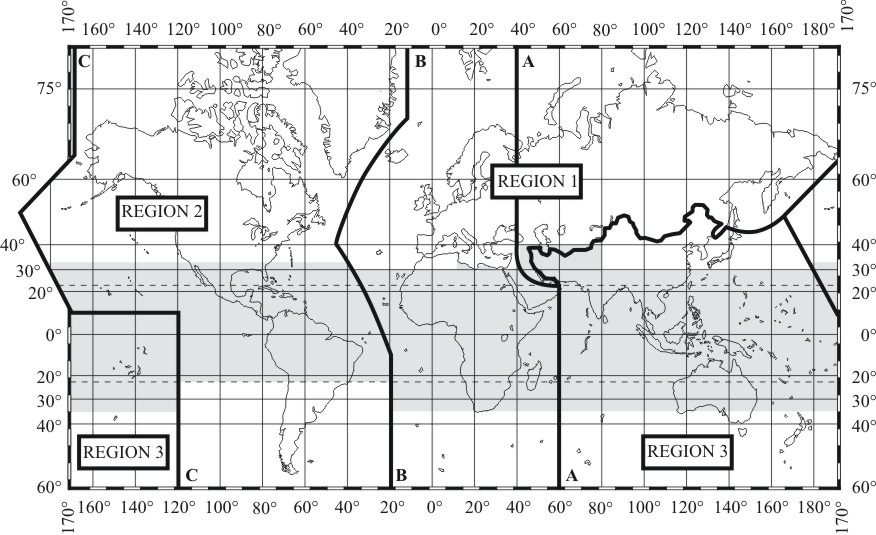
\includegraphics[width=10cm]{Capitulo2MarcoTeorico/Imagenes/ITU.png}
	\caption{División para asignación de frecuencias.}
	\caption*{Tomado del reglamento para asignaciones de frecuencia de la ITU \url{http://life.itu.ch/radioclub/image/regmap.gif}.}
	\label{fig:disitu}	
\end{figure}

\subsection{Gestión del espectro radioeléctrico en Colombia}

La gestión del espectro radioeléctrico en Colombia, es responsabilidad del estado y es un domino publico, cuya administración corresponde al Ministerio de Tecnologías de la Información y Comunicaciones (MinTIC).
\\ \\
El cuadro o tabla de asignación de frecuencias, de acuerdo a la Ley 252 de 29 de Diciembre de 1995 \cite{Ley252} y la Ley 514 de 04 de Agosto de 1999 \cite{Ley514} , corresponde al de la ITU. Este es conocido como Cuadro Nacional de Atribución de Bandas de Frecuencias.
\\ \\
Por la naturaleza dinámica de la gestión de frecuencias, el cuadro se actualiza periódicamente de acuerdo a las recomendaciones del ITU y convenios bilaterales.
\\ \\
De acuerdo a la división en regiones del mundo con respecto a la asignación del espectro, Colombia se encuentra en la Región 2.
\\ \\
En la ley 1341 del 30 de Julio de 2009 \cite{Ley1341}, se crea la Agencia Nacional del Espectro, como una unidad administrativa especial dependiente del Ministerio de Tecnologías de Información y comunicaciones, cuya función es gestionar, vigilar y controlar el espectro radioeléctrico, con excepción de los servicios de Televisión análoga y digital los cuales son administrados por la Agencia Nacional de Televisión.

\subsubsection{Cuadro nacional de atribución de frecuencias}

El cuadro nacional de atribución de frecuencias \cite{Cuadro} es un documento legal para la gestión, administración y control del espectro radioeléctrico.
\\\\
El cuadro nacional del espectro tiene las siguientes características:
\begin{itemize}
	\item Muestra todos los servicios de radiocomunicación del pais de acuerdo a la descripción de servicios de la ITU.
	\item Define la distribución del espectro radioeléctrico.
	\item Contiene referencias respecto a leyes, tratados, normas, entre otros, vinculados para el uso del espectro radioeléctrico.
\end{itemize}

Las bandas de frecuencia están definidas bajo estos conceptos:

\begin{itemize}
	\item La atribución de bandas de frecuencias a los diversos servicios de radiocomunicación comienza a partir de 9 kHz.
	\item En Colombia, la atribución nacional de frecuencias considera hasta 40,0 GHz.
	\item En Colombia, a partir de la frecuencia de 40,0 GHz y hasta la frecuencia de 1000 GHz, para fines de planeación, la atribución nacional de bandas de frecuencias es idéntica a la atribución internacional del Reglamento de Radiocomunicaciones de la ITU.
	\item La banda de frecuencias 275 - 1000 GHz no tiene actualmente atribución de servicios.
\end{itemize}

Las diferentes bandas se encuentran definidas bajo las recomendaciones de la ITU, el cuadro realiza un comparativo con la región 1, 2, 3 de la ITU con la asignación para Colombia.
\\\\
Existen dos tipos de bandas:
\begin{itemize}
	\item \textbf{Banda de frecuencia}: Estas son continuas y especifican qué servicios se presta en los diferentes bandas de frecuencia a lo largo del espectro.
	\item \textbf{Banda virtual o rango de frecuencia:} Son bandas de frecuencia definidas por servicios y con una canalización específica, es decir está dividida en segmentos los cuales pueden ser asignados, las bandas entre sí pueden solaparse o estar definidas por trozos como es el caso de la banda para el servicio de radiodifusión de televisión.
\end{itemize}

Las bandas y rangos de frecuencia pueden consultar entre las páginas 49 y 418 del cuadro nacional de atribución de frecuencias.

El cuadro nacional de atribución de frecuencias define qué servicios se prestan en el espectro radioeléctrico, los más grandes son:

\begin{itemize}
	\item \textbf{Servicio de radiocomunicación:} Todo servicio de comunicación entre un transmisor y un receptor.
	\item \textbf{Servicio Fijo:} Todos los servicios de comunicación entre estaciones fijas.
	\item \textbf{Servicio Móvil:} Agrupa los servicios que implica la comunicación con estaciones móviles.
	\item \textbf{Servicio de radioastronomía:} Son servicios aplicados a estudios en astronomía.
\end{itemize}

Los servicios pueden ser a título primario a los cuales el gobierno de Colombia se compromete a hacer respetar sus transmisiones y a título secundario los cuales pueden ser usados en una banda, pero el gobierno no garantiza que puedan ser interferidos por otros.

\subsection{Estudios económicos sobre el uso del espectro}

Para el problema de la gestión del espectro se han realizado varios estudios económicos \cite{SpectrumITU}, para estudiar el impacto de realizar una asignación determinada para una zona geográfica.
\\\\
Los costos que se deben asumir en la gestión se clasifican en:
\begin{itemize}
	\item \textbf{Costos directos:} Son los costos inmediatos de otorgar una licencia a un operador, entre los cuales se tienen, estudios de interferencia, equipos para transmisión, mover una parte congestionada del espectro y estudio de los sitios adecuados para ubicar estaciones.
	\item \textbf{Costos indirectos:} Son aquellos costos derivados de la administración del espectro, que incluye la vigilancia del uso del espectro y estudios de calidad de servicio.
\end{itemize}

Para efectos de trabajo de grado, se estudian algunos de los costos directos de la asignación del espectro los cuales son:
\begin{itemize}
	\item Costo de cambiar equipos por otros que usen mejor el espectro.
	\item Costo de mover una parte congestionada del espectro, los cuales implican el pago de compensaciones a los operadores, costos de cambio de estaciones e indemnizaciones por traumatismos para los usuarios finales.
\end{itemize}
Para efectos del trabajo de grado no se toman en cuenta los costos provocados por estudios de interferencias y ubicación de estaciones.
\\\\
Los costos indirectos no se estudian ya que son propios de la vigilancia del uso del espectro, lo que debe realizarse para garantizar se respete en la práctica la asignación realizada y es parte de los costos que no se pueden evitar en el proceso de la gestión del espectro.
\\\\
Una buena asignación del espectro busca minimizar los costos directos, buscando que la asignación sea lo más óptima posible, para evitar que se deba realizar movimiento de asignaciones para poder asignar más espectro en una banda determinada.



%%%%%%%%%%%%%%%%%%%%%%%%%%%%%%ProgramacionPorRestricciones%%%%%%%%%%%%%%%%%%%%%%%%%%%%%%%%%%%%%%%%%%%%
%\section{Programaci\'on por restricciones}

La programación por restricciones \cite{Francesca} es una herramienta poderosa para solucionar problemas combinatorios. La programación por restricciones utiliza técnicas de diferentes áreas, por ejemplo de inteligencia artificial, ciencias de la computación y lenguajes de programación. La programación por restricciones es actualmente aplicada para problemas de muchos dominios, como son la programación de tareas, planeación, búsqueda de caminos o rutas para llegar a un punto, redes de comunicación y bioinformática. 
\\ \\
La idea básica en programación por restricciones es que el usuario escriba las restricciones y un solucionador de propósito general halle una solución. Las Restricciones son relaciones y un problema de satisfacción de restricciones (CSP) contiene las relaciones entre las variables de decisión. Los modelos de restricciones, son representados en términos de variables de decisión y restricciones, a partir de ellos, se debe encontrar una asignación de todas las variables que satisfaga las restricciones. Los solucionadores para programación por restricciones buscan sistemáticamente la solución en un espacio de búsqueda, con algoritmos de \textit{Backtracking} o \textit{Branch and Bound}. El método de búsqueda sistemático busca la interpolación, se conoce como la propagación de la información contenida en una restricciones a otras restricciones, lo que reduce el espacio de búsqueda de valores para un conjunto de variables.

\subsection{Problemas de satisfacci\'on de restricciones.}

Un problema de satisfacción de restricciones \cite{Krzysztof} se define así:

\begin{itemize}
\item Variables $y_{1},y_{2},...,y_{n}$
\item Dominios  $D_{1},D_{2},...,D_{n}$
\item Restricciones  $C: y_{1} \in D_{1},y_{2} \in D_{2},...,y_{n} \in D_{n}$
\end{itemize}

Una solución es:

$$(d_{1},d_{2},...,d_{n}) \in D_{1}*D_{2}*...*D_{n}$$

Donde se cumplen las restricciones C, es decir:

$$(d_{1},d_{2},...,d_{n}) \in C $$

\subsection{Satisfacci\'on de restricciones}

La satisfacción de restricciones \cite{Francesca}, es básicamente encontrar un valor para cada una de las variables del problema. Las restricciones podan los posibles valores de las variables; para conseguir un solución al problema se utilizan estrategias de búsqueda.
\\ \\
La estrategia de búsqueda fundamental es el \textit{Backtracking} o vuelta hacia atrás, que consiste en realizar un recorrido en un árbol o grafo dirigido que no contiene ciclos. El objetivo es recorrer la estructura hasta encontrar soluciones, lo que se consigue obteniendo soluciones parciales a medida que progresa el recorrido; las soluciones parciales limitan las regiones donde se puede encontrar una solución completa. La búsqueda tiene éxito, si se puede encontrar una solución completa, el algoritmo puede detenerse o buscar soluciones alternativas. Si no encuentra una solución en un recorrido por una parte de la estructura del grafo dirigido o árbol, vuelve hacia atrás de forma similar a la de un recorrido por profundidad, eliminando los elementos que se hubieren añadido en cada fase.

\subsection{Propagaci\'on de restricciones}

La propagación de restricciones \cite{Krzysztof} es un concepto general, que consiste en encontrar relaciones entre restricciones usando algoritmos de filtrado, interferencia de restricciones, reglas de interacción e interacciones caóticas. 
\\ \\
La propagación de restricciones embebe cualquier razonamiento que consista en prohibir cualquier valor o combinación de valores para algunas variables de un problema a causa de que un subgrupo de restricciones no pueden ser satisfechas.

\subsubsection{Arco consistencia:} 

La arco consistencia es la más conocida de todas las formas de propagación de restricciones. Para que un CSP sea arco consistente se requiere que:
\\ \\
Para un conjunto de variables $X$ e $Y$, se requiere que $ \forall X \in dom(X)$ $\exists Y \in dom(Y)$ tal que $r(X,Y)$ esta satisfecha y sea recíproca, es decir para todo $\forall Y \in dom(Y) \exists x \in dom(X) $ tal que $r(X,Y)$ esta satisfecha.

\subsection{Estrategias de búsqueda}

Una estrategia de búsqueda \cite{Krzysztof} consiste en un árbol de búsqueda y un algoritmo de búsqueda el cual explorar el árbol nodo a nodo para encontrar soluciones a un problema de programación por restricciones específico. Existen dos grandes estrategias de búsqueda la \textit{Branch and Bound} y el \textit{Backtrack}.

\subsubsection{Árbol de búsqueda}

Un árbol de búsqueda está representado de la siguiente manera
\begin{figure}[H]
	\centering
	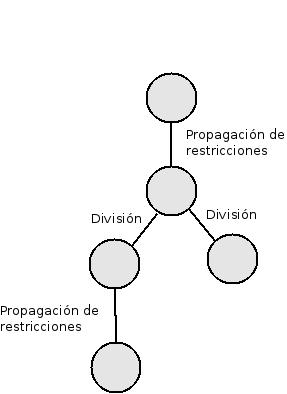
\includegraphics[width=5cm]{Capitulo2MarcoTeorico/Imagenes/Restri.jpeg}
	\caption{Estructura de un árbol de búsqueda}
	\label{fig:busqueda}	
\end{figure}

En la figura \ref{fig:busqueda} las operaciones de propagación de restricciones indican que al aplicar una restricción a un dominio finito $D$ éste se conserva o se reduce para obtener un dominio $D^{'}$. El momento en que se realizan las operaciones de división, es cuando no se puede propagar más las restricciones y el resultado es la división del dominio $D$ en $n$ dominios $D_{1}, ... ,D_{n}$


\subsubsection{Algoritmo Backtrack}

Este algoritmo construye una solución iniciando con una instancia vacía y sucesivamente intenta extender hasta obtener una instancia consistente definida por las siguientes variables. Si el procedimiento obtiene que la variable final obtiene una instanciación se encuentra una solución.
\\\\
Bajo esta premisa se han elaborado muchas estrategias de búsqueda como son \textit{Backtrack-free search with constraint propagation} y \textit{Backtrack-free Search}.
\\\\
Estas no son objeto de estudio, ya que en el proyecto se utiliza la estrategia \textit{Branch and Bound} programada en \textit{Mozart OZ}.

\subsubsection{Branch and Bound}

En este algoritmo existen dos grandes procedimientos:

\begin{itemize}
	\item \textbf{Ramificación:} La expansión del árbol de búsqueda está condicionado por la búsqueda de la mejor solución, con esto se exploran todos los nodos de una rama hasta explorar en un nuevo nivel.
	\item \textbf{Poda:} El objetivo es eliminar aquellos nodos que no lleven a soluciones buenas, con esto se busca evitar expandirlos ya que sus hijos tampoco serán buenas soluciones.
\end{itemize}

Esta es una de las mejores estrategias para realizar búsquedas ya que evita expandir todo el árbol, para obtener ganancias en velocidad de procesamiento y uso de memoria.

\subsubsection{Motores de búsqueda}

Son algoritmos que permiten filtrar las soluciones encontradas por un algoritmo de búsqueda, por ejemplo seleccionar las soluciones que mejoran un costo determinado. Con éstos motores se busca encontrar la mejor solución a un problema de acuerdo a criterios de costo propios del problema.

\subsubsection{Recomputación}

Durante el proceso de expansión de un árbol de búsqueda\cite{MultiOZ} se almacena en memoria la información de cada nodo expandido; con esto se busca evitar que se calcule de nuevo un nodo si el algoritmo de búsqueda va hacia atrás. Un nivel de recomputación $n$ indica que se almacenan los nodos que quedan a una distancia $n$ de un nodo que se encuentra guardado. La recomputación es útil para árboles de búsqueda muy grandes donde se requiere una gran cantidad de memoria para su almacenamiento pero tiene un costo adicional de procesamiento al tener que calcular de nuevo los nodos no almacenados en memoria. 

\subsection{Estrategias de distribución}

Una estrategia de distribución\cite{RestriCurso} define la forma y el contenido del árbol de búsqueda, cuántas alternativas existen en un nodo y qué restricción se agrega por cada alternativa. Las estrategias de distribución se utilizan para mejorar el rendimiento de los algoritmos de búsqueda, ya que una definición apropiada de un árbol de búsqueda permite guiar la exploración para encontrar más rápido la solución óptima.





%%%%%%%Capitulo TRES: Medición de multifractalidad%%%%%%

\chapter{Análisis de multifractalidad}\label{cap3}
\markboth{Análisis de multifractalidad}{Análisis de multifractalidad}
%\section{Alcances} 

%%%%%Capitulo CUATRO: Modelo%%%%%%%%
\chapter{Análisis de la robustez}
\markboth{Análisis de la robustez}{Análisis de la robustez}

%%%%%%%%%%%%%%%%%%%%%%%%%%%%%%Especificación del modelo%%%%%%%%%%%%%%%%%%%%%%%%%%%%%%%%%%%%%%%%%%%
%
\section{Anotaciones sobre el modelo}

La asignación en una banda se representa en una matriz de $n$ operadores por $c$ canales, donde la posición $i,j$ representa la asignación del operador $i$ en el canal $j$. La asignación se representa con un dato binario de la siguiente forma:

\begin{itemize}
	\item 0 si está libre.
	\item 1 si está asignado a un operador.
\end{itemize}

En la figura \ref{fig:ejemploAsignacion} se puede observar un ejemplo de una asignación para una banda con 9 canales y 3 operadores.

\begin{figure}[H]
	\centering
	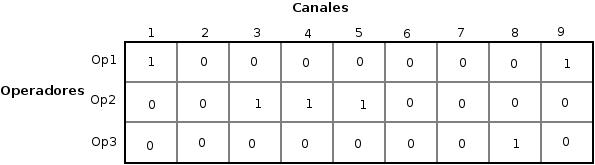
\includegraphics[width=11cm]{Capitulo4Modelo/Imagenes/Ejemplo.jpeg}
	\caption{Ejemplo de representación de asignación en una banda.}
	\label{fig:ejemploAsignacion}	
\end{figure}



\section{Datos de entrada}

Las variables de entrada representan el estado actual del modelo, en otras palabras la asignación actual del espectro en una banda de interés.

\begin{itemize}
	\item $C$: Cardinalidad del conjunto de canales definidos para un servicio particular.
	\item $O$: Número de operadores en la banda que requieren asignación.
	\item $N$: Número de operadores presentes en la banda.
	\item $OPp = \{o_k: 1 \leq k \leq N\}$: Conjunto de etiquetas que representan a los operadores presentes.
	\item $OPi = \{o_k: 1 \leq k \leq O\}$: Conjunto de etiquetas que representan a los operadores que solicitan canales. Si $o_k \in OPp$, es un operador presente o antiguo; sino, es un operador nuevo.
	\item $OPt$ = $OPp \cup OPi$: Son las etiquetas de los operadores presentes en la banda y de los que requieren asignación.
	\item $CI_{c} \in \{0,1\}$: Canales marcados como inutilizables en la banda, si $CI_{c} = 1$ el canal $c$ es inutilizable, en caso contrario se puede usar, donde  $1 \leq c \leq C$.
	\item $CR_{c} \in \{0,1\}$: Canales marcados como reservados en la banda,  si $CR_{c} = 1$ el canal $c$ está reservado, en caso contrario se puede usar, donde  $1 \leq c \leq C$.
	\item $CP_{c} \in \{0,1\}$: Canales asignados en las subdivisiones de la banda,  si $CP_{c} = 1$ el canal $c$ está asignado, en caso contrario se encuentra libre, donde  $1 \leq c \leq C$.
	\item $B^{I}_{co} \in \{0,1\}$: Indica si en el canal $c$ de la banda se encuentra asignado el operador $o$ donde $1 \leq c \leq C, o \in OPp$.
	\item $Req=[(o_{1}, nr_{1}), (o_{2}, nr_{2}), ... ,(o_{O}, nr_{O})]$: $(o, nr)$ indica que el operador etiquetado $o \in OPi$ requiere $nr$ canales.
	\item $Sep$: Valor de separación mínima de canales entre canales asignados a operadores distintos.
	\item $Tope$: Valor máximo de canales que puede tener asignado un operador en una banda específica.
	\item $AP_{o}$: Indica el número máximo de canales que tiene el operador $o$ en una subdivisión de la región de trabajo, donde $1 \leq o \leq O$.
	\item $R$: Número máximo de operadores por canal. Por defecto su valor es 1.
	\item $CAC \in \{0,1\}$: Indica si se conserva asignación para operadores que solicitan nuevos canales y ya tienen asignación actualmente.
\end{itemize}


\section{Variables de decisión}

Las variables de decisión son aquellas que se desean encontrar en el problema, en este caso la asignación de canales a nivel nacional, regional, departamental o municipal.

\begin{itemize}
	\item ${B}^{O}_{co} \in \{0,1\}$ Asignación de los operadores en la banda, donde $1 \leq c \leq C, o \in OPt$
\end{itemize}


\section{Variables usadas en restricciones y estrategias de búsqueda}

Son aquellas variables que se utilizan para ayudar a definir algunas restricciones y las estrategias de búsqueda.

\begin{itemize}
	\item{$EC_{c} \in \{0,1\}$ es una variable reificada que define si el canal $c$ esta libre u ocupado.
	\begin{displaymath}
		\begin{array}{cc}
			(\forall c \in \{1,2,...,C\} ) \sum \limits_{o \in OPt} B^{O}_{co} + CP_{c} < 1 \leftrightarrow EC_{c} = 1
		\end{array}
	\end{displaymath}
	El canal $c$ se encuentra libre si y sólo si $EC_{c} = 1$}
	\item {$CAO_{co} \in \{0,1\}$: Permite conocer el número de bloques contiguos asignados a un operador $o$, de la siguiente forma:
	\begin{displaymath}
		CAO_{co} = \left\{ \begin{array}{lp{5cm}} 1  \textrm{ Si un bloque de canales asignados al operador etiquetado $o$ termina en el canal $c-1$ } \\1 \textrm{ Si un bloque de canales asignados al operador etiquetado $o$ inicia en el canal $c$ } \\0 \textrm{ En otro caso}\end{array}\right.
	\end{displaymath}	
	Si para un operador $o$ se cumple $B^{O}_{co} \neq B^{O}_{(c+1)o}$ y $c<C$ entonces $CAO_{co}=1$ en caso contrario $CAO_{co}=0$, para el caso donde $c=C$ y $B^{O}_{co}=1$ entonces $CAO_{co}=1$ en caso contrario $CAO_{co}=0$, donde: $1 \leq c \leq C, o \in OPt$.}
	\item $CLM_{c}$: Define el tamaño de los bloques libres, si $c=1$ entonces $CLM_{c}=EC_{c}$, si $c>1$ y $EC_{c}=1$ entonces  $CLM_{c}=1+CLM_{c-1}$, si $c > 1$ y $EC_{c}=0$  entonces $CLM_{c}=0$, donde $1 \leq c \leq C$.
	\item $CLMmax = max(CLM_c: 1 \leq c \leq C)$
	\item {$CAI_{c} \in \{0,1\}$: Permite conocer que canales se encuentran marcados como inutilizados debido a la separación mínima exigida entre dos operadores diferentes.
	\begin{displaymath}
		CAI_{c} = \left\{ \begin{array}{lp{5cm}} 1  \textrm{ Si el canal se encuentra a una distancia entre $1$ y $Sep$ de un canal asignado} \\0 \textrm{ En otro caso } \end{array}\right.
	\end{displaymath}		
	Para un canal $c$ y un operador $o$ si $B^{O}_{co}=1$ y $B^{O}_{(c+1)o}=0$, entonces $\forall c, 1 \leq i \leq Sep, CAI_{c+i}= 1$, en caso de que $B^{O}_{co}=1$ y $B^{O}_{(c-1)o}=0$ entonces  $\forall c, 1 \leq i \leq Sep, CAI_{c-i} = 1$, si $B^{O}_{co} = B^{O}_{(c+1)o}$ entonces $CAI_{c}=0$  . En caso de que $R>1$ o $Sep=0$, entonces $\forall c \in \{1,2,...,C\} , CAI_{c}=0$}
\end{itemize}


\section{Restricciones}

\subsection{Restricciones triviales}


Todo operador que solicita canales y actualmente tiene canales asignados los conserva a menos que $CAC \neq 1$

\begin{equation}
	\begin{array}{cc}
		CAC = 1 \to \forall c \in \{1,2,...,C\} ,o \in OPp \cap OPi, B^{I}_{co} = 1 \to  B^{O}_{co} = 1
	\end{array}
\end{equation}

Todo operador que no solicita canales tendrá la misma asignación de canales en la salida

\begin{equation}
	\begin{array}{cc}
		\forall c \in \{1,2,...,C\} , o \in OPp \setminus OPi\\
		B^{I}_{co} = B^{O}_{co}
	\end{array}
\end{equation}

Máximo R operadores por canal

\begin{equation}
	\begin{array}{cc}
		\forall c \in \{1,2,...,C\}  \sum \limits_{o \in OPt} B^{O}_{co} + CP_{c} \leq R
	\end{array}
\end{equation}

En el caso de que un canal esté reservado o marcado como inutilizable, no puede ser asignado a ningún operador que requiere asignación

\begin{equation}
	\begin{array}{cc}
		\forall c \in \{1,2,...,C\} CI_{c} + CR_{c} \geq 1 \to \sum \limits_{o \in OPi} B^{O}_{co} = 0
	\end{array}
\end{equation}

Todos los operadores que solicitan canales y no se encuentran actualmente con asignación, deben tener asignados un número de canales igual al que requieren.

\begin{equation}
	\begin{array}{cc}
		\forall o \in OPi \setminus OPp, \sum \limits^{C}_{c=1} B^{O}_{co} = Req_{o}
	\end{array}
\end{equation}

Todos los operadores que solicitan canales y actualmente tienen asignación, deben tener asignados un número de canales igual al que requieren más los canales que actualmente poseen en la banda.

\begin{equation}
	\begin{array}{cc}
		\forall o \in OPi \cap OPp, \sum \limits^{C}_{c=1}B^{O}_{co} = \sum \limits^{C}_{c=1}B^{I}_{co} + Req_{o}
	\end{array}
\end{equation}

\subsection{Restricciones co-canal}

Debe existir una distancia de $Sep$ entre dos canales asignados a operadores diferentes que solicitan asignación.

\begin{equation}
	\begin{array}{cc}
	R=1 \to (\forall o \in OPi, \forall o' \in OPt, \forall s \in \{1,2,...,Sep\}, \forall c \in \{1,2,...,C\} , o \neq o')\\(B^{O}_{co}+B^{O}_{(c \pm s)o'} \leq 1)
	\end{array}
\end{equation}

\subsection{Restricciones legales}

Un operador no puede superar el tope de canales establecido por el gobierno en una banda de la región ni en sus divisiones territoriales

\begin{equation}
	\begin{array}{cc}
	(\forall o \in OPi)\sum \limits^{C}_{c=1} B^{O}_{co} + APo_{o} \leq Tope
	\end{array}
\end{equation}




%%%%%%%%%%%%%%%%%%%%%%%%%%%%%%Cálculo de costos%%%%%%%%%%%%%%%%%%%%%%%%%%%%%%%%%%%%%%%%%%%%%%%%%%%
%
\section{Cálculo de costos}

\subsection{Número de cambios de asignación de canales para un operador}

Los cambios en los canales asignados a un operador $Cost_{1}$, se calcula de acuerdo a la ecuación \ref{equ:costoNb}

\begin{equation}
	\label{equ:costoNb}
	\begin{array}{cc}
		Cost_{1} = \lceil\frac{1}{2}*\sum \limits_{o \in OPi} \sum \limits^{C}_{c=1} CAO_{co}\rceil	
	\end{array}
\end{equation}

Se toma como el número de bloques la mitad del cálculo realizado en $CAO_{co}$ ya que este cuenta los limites de cada bloque, es decir que para un bloque se cuenta su inicio y su final, por lo que si hay $n$ bloques se contarán $2n$ en $CAO_{co}$; sin embargo en el caso de que el primer bloque inicia en la posición $1$ de la banda, no se cuenta, por lo que se toma el techo de este cálculo, ya que en ese caso da un número impar.

\subsubsection{Justificación}

El número de cambios en la asignación de un operador representa costos adicionales en la práctica ya que debe adquirir equipos adicionales para trabajar en canales que se encuentran separados. Por lo tanto, es ideal dar a un operador un bloque contiguo en la asignación para reducir costos.

\subsection{Diferencia entre el número de canales y el mayor bloque de canales libres}

La diferencia entre el número de canales de una banda y el tamaño del mayor bloque libre $Cost_{2}$ se calcula de acuerdo a la ecuación \ref{equ:cost2}.

\begin{equation}
	\label{equ:cost2}
	\begin{array}{cc}
		Cost_{2} = C - CLMmax
	\end{array}
\end{equation}

\subsubsection{Justificación}

Se busca que la asignación en una banda considere dejar un bloque de canales libres, para facilitar la asignación en futuros requerimientos, debido a que no se conoce cuantos canales se van a necesitar y se desea realizar la mejor asignación posible para esos requerimientos.

\subsection{Número de canales inutilizables}

Un canal libre es marcado como inutilizable cuando no puede ser asignado a ningún operador debido a la separación mínima exigida. En la ecuación \ref{equ:cost3} se muestra cómo calcular este costo.

\begin{equation}
	\label{equ:cost3}
	\begin{array}{cc}
			Cost_{3} = \sum \limits^{C}_{c=1} CAI_{c}
	\end{array}
\end{equation}

\subsubsection{Justificación}

En la asignación se debe buscar que el número de canales inutilizados por la separación sea la mínima posible debido a que esto representa un desperdicio de canales que no pueden ser asignados.

\subsection{Costo total}

El costo total se calcula a partir de la suma de pesos entre 1 y 100 especificados por el usuario conocidos como $peso_{1}, peso_{2}, peso_{3}$ multiplicado por cada uno de los costos.

\begin{equation}
	\label{equ:costR}
	\begin{array}{cc}
		Cost_{T} = peso_{1}*Cost_{1} + peso_{2}*Cost_{2} + peso_{3}*Cost_{3}
	\end{array}
\end{equation}


%%%%%%%%%%%%%%%%%%%%%%%%%%%%%%Justificacion Modelo%%%%%%%%%%%%%%%%%%%%%%%%%%%%%%%%%%%%%%%%%%%%%%%%%%%%
%\section{Justificación del modelo}

\subsection{Uso de matrices y codificación binaria de dominios}

El uso de matrices permite modelar con más precisión algunas restricciones, como es el caso de la separación y posibilita que el canal este asignado a más de un operador a diferencia del caso de una lista de canales.
\\\\
El uso de dominios binarios permite modelar con mayor facilidad las restricciones de tope, separación entre operadores diferentes y de no asignar en canales marcados como asignados y reservados. Además hace posible el uso de marcadores para los canales como reservado, inutilizado y asignado en división sin hacer uso de artilugios propios de la implementación, como codificarlos como operadores virtuales. 

\subsection{Tipos de restricciones}

Los tipos de restricciones han sido extraídos de la solución al problema de \textit{channel assigment} \cite{Hurley} y del uso de topes por operador por parte del gobierno nacional colombiano \cite{Tope}.
\\\\
Se definen los tipos de restricciones así:

\begin{itemize}
	\item \textbf{Restricciones co-canal:} Son aquellas restricciones aplicadas a transmisores ubicados dentro de una pequeña zona, se asume en el modelo que un operador tiene transmisores en toda una zona geográfica, por lo tanto se debe garantizar una separación entre dos operadores diferentes.
	\item \textbf{Restricciones triviales:} Garantizan que se respete la asignación actual de los operadores, las asignaciones no se pueden mover en principio por los enormes costos que se generan en ese proceso.
	\item \textbf{Restricciones legales:} La única restricción que se toma es la de topes por operador, no se evalúa calidad de servicio ni potencia de emisiones, eso es objeto de estudio futuro. 
\end{itemize}

\subsection{Limitaciones de encontrar soluciones óptimas}

Con el modelo se pueden obtener soluciones óptimas para la asignación en una zona determinada, pero no en cada una de las divisiones de esa zona. Por ejemplo, para el caso de los departamentos la asignación obtenida a nivel departamental cumplirá todas las restricciones y tendrá el mejor costo, pero no necesariamente es así para los municipios que componen el departamento ya que al no considerar el detalle, un operador puede quedar con una asignación con un peor costo que la solución óptima considerando cada uno de los municipios.
\\\\
Esta decisión fue tomada debido al gran tamaño que tomaban las entradas al considerar el detalle de las divisiones territoriales, dificultaban su lectura y manejo en el aplicativo, además complica enormemente el modelado del problema ya que las restricciones deben considerar las asignaciones en cada una de las divisiones de la zona geográfica. En su lugar se ha optado por marcar los canales como asignados si alguna de las divisiones del territorio está asignado.



%%%%%Capitulo CINCO: Implementacion%%%%%%%%
\chapter{Implementación de la librería} \label{capimp}
\markboth{Implementación de la librería}{Implementación de la librería}

%%%%%%%%%%%%%%%%%%%%%%%%%%%%%%%%%Introducion%%%%%%%%%%%%%%%%%%%%%%%%%%%%%%%%%%%%%%%%%%%%%%%%%%%%%%%%%%%%%%%
%Para realizar el proceso de implementación del proyecto se deben tomar en cuenta los pasos especificados en la metodología para aplicaciones Web del grupo Avispa \cite{Metodologia}.
\\\\
En este capítulo se dan las pautas más relevantes para la implementación de la aplicación que son:

\begin{itemize}
	\item Formatos de entradas y salidas.
	\item Parámetros de las aplicaciones.
\end{itemize}

Para facilitar la divulgación del proyecto, la aplicación se nombra cómo: \textbf{CaFeSA} que es la abreviación de \textit{Constraints Application For Enhanced Spectrum Allocation}, en español, aplicación por restricciones para asignación de espectro aumentado.


%%%%%%%%%%%%%%%%%%%%%%%%%%%%%%%%%%Formatos E/S%%%%%%%%%%%%%%%%%%%%%%%%%%%%%%%%%%%%%%%%%%%%%%%%%%%%%%%%%%%%%
%\section{Formato de entradas} 

A continuación se va definir el formato de las entradas para los aplicativos del proyecto, un ejemplo de entrada puede ser consultado en el anexo entradas de ejemplo ubicado en la página \pageref{ejemploEntrada}.

\subsection{Formato general}
Para las entradas se utiliza el formato XML usando la especificación \textit{dict} de XCSP\cite{XCSP}.
\\\\
Para definir una entrada de acuerdo al formato \textit{dict}, se debe asociar un orden convencional a un diccionario. Este orden convencional especifica un orden de llaves que pueden ser usadas para acortar notaciones. Mientras el grupo de llaves pueda ser conocido desde el contexto, los valores de cada llave pueden ser escritos en una notación abreviada, listando los valores de cada llave que son conocidas en el diccionario.
\\\\
Por ejemplo, las coordenadas de un punto pueden ser representadas por un diccionario que contiene dos llaves $x$ e $y$ con valores (2,5) respectivamente.

\lstset{frameround=fttt}
\begin{lstlisting}[frame=trBL, language=XML]
<dict>
<entry key="x"><i>2</i></entry>
<entry key="y"><i>5</i></entry>
</dict>
\end{lstlisting}
\subsection{Especificación de llaves}
Para el proyecto se han definido las siguientes llaves:

\begin{center}
\begin{longtable}{|p{7cm}|p{9cm}|}
	\caption{Estructura de llaves en las entradas}\\
	\hline
	\cellcolor[gray]{0.9} \textbf{Llave} & \cellcolor[gray]{0.9}\textbf{Descripción} \\
	\hline
	GeograficAssignationType & Tipo de asignación geográfica, 0 indica nacional, 1 territorial o regional, 2 departamental y 3 municipal.\\
	\hline
	GeograficAssignationID & ID o llave de la entidad territorial, en el caso de asignación nacional este valor es 0.\\
	\hline
	FrequencyBand & ID o llave banda de frecuencia de trabajo. \\
	\hline
	FrequencyRank & ID o llave del rango de frecuencia o banda específica de trabajo.\\
	\hline
	NumberChannels & Número de canales que tiene la canalización del rango de frecuencia.\\
	\hline
	NumberPresentOperators & Número de operadores que tienen asignación actualmente en el rango de frecuencia.\\
	\hline
	NumberOfOperatorWithRequirements & Número de operadores que requieren asignación.\\
	\hline
	ChannelSeparation & Separación mínima de canales entre dos operadores diferentes.\\
	\hline
	PresentOperators & Lista de operadores que tienen asignación en la banda actualmente.\\
	\hline
	OperatorsWithRequeriments & Lista de operadores que requieren asignación.\\
	\hline
	Requeriments & Lista de los requerimientos en canales que tienen los operadores que requieren asignación.\\
	\hline
	MaxAssignationsSubDivision & Lista que indica el máximo número de canales que tiene asignado en una división del área geográfica cada operador que solicita asignación.\\
	\hline
	ChannelAssignInDivisions & Indica que canales están asignados en las divisiones del área geográfica.\\
	\hline
	ReservedChannels & Indica que canales están reservados en las divisiones del área geográfica.\\
	\hline
	DisabledChannels & Indica que canales están deshabilitados en las divisiones del área geográfica.\\
	\hline
	ChannelAssignation & Matriz que especifica la asignación actual para los operadores presentes.\\
	\hline
	MaxChannelAssignationByOperator & Indica el máximo número de canales que puede tener asignado un operador en la banda.\\
	\hline
\end{longtable}	
\end{center}



%
\section{Formato de salidas} \label{sec:formatSal}

A continuación se definen la estructura de salidas que se va a utilizar en el aplicativo, un ejemplo puede ser consultado en el anexo salida de ejemplo ubicado en la página \pageref{ejemploSalida}.

\subsection{Formato general}

A partir de la metodología la estructura de la salida XML es la siguiente:

\begin{enumerate}
	\item{Raíz del documento:

	\lstset{frameround=fttt}
	\begin{lstlisting}[frame=trBL, language=XML]
	<solutions>
	</solutions>
	\end{lstlisting}}

	\item{Se establece un encabezado donde se encuentra la información de la ejecución de la aplicación:

	\lstset{frameround=fttt}
	\begin{lstlisting}[frame=trBL, language=XML]
	<head>
	</head>
	\end{lstlisting}}
	
	\item{Se estructura cada solución encontrada de la siguiente forma:

	\lstset{frameround=fttt}
	\begin{lstlisting}[frame=trBL, language=XML]
	<solution id="n">
	</solution>
	\end{lstlisting}}	
	
	$n$ indica el número de la solución, estas se encuentran ordenadas de acuerdo al mejor costo.

	\item{Se colocan los costos de cada solución y el reporte de la salida.

	\lstset{frameround=fttt}
	\begin{lstlisting}[frame=trBL, language=XML]
	<solution>
		<costs>
			...
		</costos>
		<report>
			...
		</report>
	</solution>
	\end{lstlisting}}
\end{enumerate}

Los campos de información de ejecución permiten evaluar el desempeño de la aplicación.

\begin{center}
\begin{longtable}{|p{7cm}|p{7cm}|}
	\caption{Campos de información de ejecución en general.}\\
	\hline
	\cellcolor[gray]{0.9} \textbf{Campo} & \cellcolor[gray]{0.9}\textbf{Descripción} \\
	\hline
	numSolutions & Número de soluciones encontradas.\\
	\hline
	memoryUsage & Uso del memoria del aplicativo.\\
	\hline
	executionTime & Tiempo de ejecución.\\
	\hline
\end{longtable}	
\end{center}

Los campos propios de la aplicación de programación por restricciones describen algunos aspectos de la ejecución usando programación por restricciones.
\newpage
\begin{center}
\begin{longtable}{|p{7cm}|p{9cm}|}
	\caption{Campos de información de ejecución usando programación por restricciones.}\\
	\hline
	\cellcolor[gray]{0.9} \textbf{Campo} & \cellcolor[gray]{0.9}\textbf{Descripción} \\
	\hline
	considerTop & Indica si se considera la restricción del tope de canales en la ejecución.\\
	\hline
	staticAssignation & Especifica si la asignación de canales de los operadores que requieren asignación se mantiene.\\
	\hline
	considerSeparation & Muestra si en la ejecución se ha tomado en cuenta la separación de canales de operadores diferentes.\\
	\hline
	spacesCreated & Número de espacios computacionales creados en la ejecución.\\
	\hline
	spacesSucceeded & Número de espacios computacionales exitosos en la ejecución.\\
	\hline
	FDVariables & Número de variables de estado finito creadas en la ejecución.\\
	\hline
	propagators & Número de propagadores creados durante la ejecución.\\
	\hline
\end{longtable}	
\end{center}

\subsection{Campos de una solución}

En el reporte de una solución tiene dos campos de información; el primero que son los costos de la solución y el segundo que es el reporte de la solución.

\subsubsection{Campos de los costos de una solución}

\begin{center}
\begin{longtable}{|p{7cm}|p{9cm}|}
	\caption{Campos de costos de una solución.}\\
	\hline
	\cellcolor[gray]{0.9} \textbf{Campo} & \cellcolor[gray]{0.9}\textbf{Descripción} \\
	\hline
	blocksNumber & Número de bloques existentes en la solución.\\
	\hline
	difChannelNumberMaxBlockFree & Diferencia entre el tamaño del bloque libre más grande y el número de canales.\\
	\hline
	channelNumberUseless & Número de canales inutilizados por separación.\\
	\hline
	totalCost & Costo total de la solución, que consiste en sumar los anteriores costos multiplicados cada uno por un peso especificado por el usuario.\\
	\hline
	violations & Número de violaciones a las restricciones. \textbf{Sólo aplica en algoritmo genético}.\\
	\hline
\end{longtable}	
\end{center}

\subsubsection{Campos de reporte de una solución}

\begin{center}
\begin{longtable}{|p{7cm}|p{9cm}|}
	\caption{Campos de información de un reporte de una solución específica.}\\
	\hline
	\cellcolor[gray]{0.9} \textbf{Campo} & \cellcolor[gray]{0.9}\textbf{Descripción} \\
	\hline
	operator & Indica cual es la asignación del operador.\\
	\hline
	channels & Asignación final para un operador dado.\\
	\hline
\end{longtable}	
\end{center}



%%%%%%%%%%%%%%%%%%%%%%%%%%%%%%Parametros aplicacion%%%%%%%%%%%%%%%%%%%%%%%%%%%%%%%%%%%%%%%%%%%%%%%%%%%%%%%
%\section{Parámetros de las aplicaciones}

Los parámetros de las aplicaciones se especifican así:

\begin{center}
\begin{longtable}{|p{4cm}|p{11cm}|}
	\caption{Parámetros generales para la aplicación}\\
	\hline
	\cellcolor[gray]{0.9} \textbf{Parámetro} & \cellcolor[gray]{0.9}\textbf{Descripción} \\
	\hline
	$--file$ & Ruta del archivo de entrada.\\
	\hline
	$--o$ & Ruta archivo de salida.\\
	\hline
	$--tm$ & Tiempo de ejecución máximo de la aplicación.\\
	\hline
	$--pnb$ & Peso del costo número de bloques.\\
	\hline
	$--psm$ & Peso del costo diferencia entre número de canales y el tamaño del bloque más grande libre.\\
	\hline
	$--pnc$ & Peso del costo de número de canales inutilizados.\\
	\hline
	$--ns$ & número máximo de soluciones que se escriben en la salida \\
	\hline
\end{longtable}	
\end{center}



%%%%%%%%%%%%%%%%%%%%%%%%%%%%%%%%%Base de datos%%%%%%%%%%%%%%%%%%%%%%%%%%%%%%%%%%%%%%%%%%%%%%%%%%%%%%%%%%%%
%\section{Información del cuadro nacional de atribución de frecuencias.}

Para realizar la gestión del espectro se debe sistematizar el cuadro nacional de atribución de frecuencias \cite{Cuadro}; en este proyecto se realizan los siguientes tareas para realizar éste proceso.

\begin{enumerate}
	\item Abstracción del cuadro nacional nacional de atribución de frecuencias tomando en cuenta los alcances del proyecto definidos en el capítulo \ref{cap3}.
	\item Diseño de la base de datos de acuerdo a la abstracción del cuadro nacional de atribución de frecuencia.
	\item Creación de datos de prueba para la aplicación prototipo.
\end{enumerate}

\subsection{Abstracción.}

De acuerdo a los alcances del proyecto, se abstrae el cuadro nacional de atribución de frecuencias \cite{Cuadro} bajo las siguientes consideraciones:

\begin{itemize}
	\item Se utilizan los rangos de frecuencia definidos por servicios en el cuadro nacional de atribución de frecuencias, excepto para servicios marítimo móvil y fijo.
	\item Se emplean las grandes bandas de frecuencia HF, VHF, UHF, SHF, EHF para agrupar los diferentes rangos de frecuencia de acuerdo a su frecuencia inicial.
	\item La asignación es jerárquica territorialmente, es decir que una asignación nacional aplica en todo el territorio colombiano, una departamental en sus municipios y así sucesivamente.
	\item Para la división territorial se toma en cuenta las estaciones monitoras fijas del cuadro nacional de atribución de frecuencias y la organización territorial de Colombia \cite{OrgDANE} tomando la estructura de departamentos y municipios.
\end{itemize}

\subsection{Diseño de la base de datos.}

Para el diseño de la base de datos se toma en cuenta lo siguiente:

\begin{itemize}
	\item Los rangos de frecuencias son elementos de los grandes bandas de frecuencia. Cada rango tiene autorizado uno o más servicios.
	\item Los canales son elementos de los rangos de frecuencia.
	\item Una asignación es una entidad especializada por tipo: nacional, territorial, departamental y municipal.
	\item Para determinar una asignación en una entidad territorial debe tomarse en cuenta las asignaciones en las entidades a las cuales ésta pertenece hasta llegar a las asignaciones nacionales.
	\item Los operadores prestan uno o más servicios.
\end{itemize}

De acuerdo a lo anterior, se define el modelo entidad relación de la base de datos, el cual puede se consultando en el anexo modelo entidad relación en la página \pageref{modER}.

\subsection{Datos de prueba en la aplicación prototipo.}

En la tabla \ref{dataPrueba} se muestran los diferentes datos que se encuentran la base de datos y su fuente, es de anotar que algunos son aleatorios, por la imposibilidad de obtenerlos de la ANE.

\begin{center}
\begin{longtable}{|p{7cm}|p{9.5cm}|}
	\caption{Datos de prueba de la aplicación prototipo} \label{dataPrueba} \\
	\hline
	\cellcolor[gray]{0.9} \textbf{Dato} & \cellcolor[gray]{0.9}\textbf{Fuente} \\
	\hline
	Bandas de frecuencia & Cuadro nacional de atribución de bandas de frecuencias página 47.\\
	\hline
	Rangos de frecuencia & Cuadro nacional de atribución de bandas de frecuencias páginas 246-253,272-275 y 279-418.\\
	\hline
	Servicios & Cuadro nacional de atribución de bandas de frecuencias páginas 23-27.\\
	\hline
	Servicios por rango de frecuencia & Cuadro nacional de atribución de bandas de frecuencias páginas 51-141.\\
	\hline
	Operadores & Operadores concodios que utilizan el espectro conocidos en Colombia que prestan servicios en el espectro.\\
	\hline
	Servicios por operador & Ninguna.\\
	\hline
	Tope por operador en rango de frecuencia & Ninguna.\\
	\hline
	Separación en rango de frecuencia & Ninguna.\\
	\hline
	División territorial o regiones & Para las regiones se utiliza la definición del cuadro nacional de atribución de bandas de frecuencias en el anexo II estaciones monitoras fijas.\\
	\hline
	Lista de departamentos y municipios & Biblioteca virtual del Banco de la República de Colombia \cite{ListMunDep}, actualizada al 2005. \\
	\hline
	Asignación actual & Ninguna. \\
	\hline
\end{longtable}	
\end{center}



%%%%%%Capitulo SEIS: Análisis comparativo%%%%%%%%%%%%%%%%%%%%%
\chapter{Análisis comparativo}\label{cap6}
\markboth{Análisis comparativo}{Análisis comparativo}

%%%%%%%%%%%%%%%%%%%%%%%%%%%%%%%%%Introduccion%%%%%%%%%%%%%%%%%%%%%%%%%%%%%%%%%%%%%%%%%%%%%%%%%%%%%%%%%%%%
%En este capítulo se muestran los aspectos más relevantes del proceso de implementación. Se explican qué estrategias de búsqueda y distribución se usaron, la estructura del aplicativo y se realizan algunos apuntes con respecto al proceso de implementación que deben ser tenidos en cuenta al momento de utilizar la aplicación.
\\\\
Las estrategías de búsqueda y distribución son propias del proceso de programación por restricciones, donde se busca mejorar el proceso de ejecución del aplicativo para encontrar las soluciones óptimas más rapidamente. 
\\\\
La flexiblidad y debilidad en las restricciones permite encontrar soluciones en instancias del problema que no cumplen las restricciones. A lo largo de éste capítulo se decribe cómo se implementaron.


%%%%%%%%%%%%%%%%%%%%%%%%%%%%%%%%%Estrategias distribución%%%%%%%%%%%%%%%%%%%%%%%%%%%%%%%%%%%%%%%%%%%%%%%%%
%
\section{Estrategias de distribución}

Las estrategias de distribución están enfocadas a mejorar el rendimiento del algoritmo de búsqueda y están diseñadas para agilizar el proceso de gestión del espectro a partir de conocer las características propias de una banda específica. Por ejemplo, si esta se encuentra ocupada al inicio, lo más recomendable es intentar asignar al inicio, ya que la mejor solución de acuerdo a los costos definidos en el modelo buscan que los bloques libres sean lo más grandes posibles.\\

Para definir las estrategias de distribución se crean las siguientes variables auxiliares:

\begin{itemize}
	\item $Req$ es la lista de requerimientos, es una lista de tuplas que contiene los elementos $(o_{i}, nr_{i})$ donde $o_{i}$ es el operador $i$ y $nr_{i}$ es el número de canales requeridos por el operador $i$.
	\item $ReqA$: Es una sublista de $req$ que contiene los requerimientos correspondientes a los operadores que ya tienen asignación en la banda. Es decir que $o_{i} \in OPi \cap OPp$.
	\item $NReqA$: Es una sublista de $req$ que contiene los requerimientos correspondientes a los operadores que no tienen asignación en la banda. Es decir que $o_{i} \in OPi \setminus OPp$.
	\item $MayorReq$: es la lista de requerimientos ordenada de mayor a menor de acuerdo al número de canales solicitados por cada operador.
	\item $MenorReq$: es la lista de requerimientos ordenada de menor a mayor de acuerdo al número de canales solicitados por cada operador.
\end{itemize}


En la tabla \ref{table:esDistribucion} se especifican los diferentes estrategias de distribución usados en el proyecto.

\begin{center}
\begin{longtable}{|p{3cm}|p{13.5cm}|}
	\caption{Estrategias de distribución} \label{table:esDistribucion}\\
	\hline
	\cellcolor[gray]{0.9} \textbf{Estrategia} & \cellcolor[gray]{0.9}\textbf{Descripción} \\
	\hline
	Asignar primero al inicio de la banda & Se toman los requerimientos $Req$ en orden de llegada, se toma el primer requerimiento y se intenta asignar en el primer canal de la banda, si no es posible en el segundo y así sucesivamente; una vez se ha cumplido el primer requerimiento se prosigue con el segundo hasta tomar todos los requerimientos.\\
	\hline
	Asignar primero al final de la banda & Se toman los requerimientos $Req$ en orden de llegada, se toma el primer requerimiento y se intenta asignar en el último canal de la banda, si no es posible en el penúltimo y así sucesivamente; una vez se ha cumplido el primer requerimiento se prosigue con el segundo hasta tomar todos los requerimientos.\\
	\hline
	Asignar primero a operadores en orden de llegada con asignación al inicio de la banda &  Se intenta asignar canales al inicio de la banda a la lista de requerimientos $ReqA$ y luego a $NReqA$.\\
	\hline
	Asignar primero a operadores en orden de llegada con asignación al final de la banda &  En este caso se asignar canales al final de la banda a la lista de requerimientos $ReqA$ y luego a $NReqA$.\\
	\hline
	Asignar primero a operadores sin asignación al inicio de la banda & En este caso se asignar canales al inicio de la banda a la lista de requerimientos $NReqA$ y luego a $ReqA$.\\
	\hline
	Asignar primero a operadores sin asignación al final de la banda & En este caso se asignar canales al final de la banda a la lista de requerimientos $NReqA$ y luego a $ReqA$.\\
	\hline
	Asignar primero a requerimientos más grandes al inicio de la banda & A partir de $MayorReq$ se realiza el proceso de asignación intentado asignar a partir del inicio de la banda.\\
	\hline
	Asignar primero a requerimientos más grandes al final de la banda & A partir de $MayorReq$ se realiza el proceso de asignación intentado asignar a partir del final de la banda.\\
	\hline
	Asignar primero a requerimientos más pequeños al inicio de la banda & A partir de $MenorReq$ se realiza el proceso de asignación intentado asignar a partir del inicio de la banda.\\
	\hline
	Asignar primero a requerimientos más pequeños al final de la banda & A partir de $MenorReq$ se realiza el proceso de asignación intentado asignar a partir del final de la banda.\\
	\hline
	Estrategia genérica: ff & Intenta asignar la primera variable de la lista, donde el domino es más pequeño, por el menor valor del dominio es decir 0.\\
	\hline
	Estrategia genérica: naive  & Intenta asignar la primera variable de la lista, por el menor valor del dominio es decir 0.\\
	\hline
	Estrategia genérica: split  & Intenta asignar la primera variable de la lista, por el valor medio del dominio es decir 1.\\
	\hline
\end{longtable}	
\end{center}


%%%%%%%%%%%%%%%%%%%%%%%%%%%%%%%%%Estrategias búsqueda%%%%%%%%%%%%%%%%%%%%%%%%%%%%%%%%%%%%%%%%%%%%%%%%%%%%%
%\section{Estrategias de búsqueda} \label{sec:esbusq}

Las estrategias de búsqueda utilizadas en el aplicativo se muestran en la tabla \ref{table:esBusqueda}. La función objetivo en los costos consiste en encontrar la solución con el costo mínimo.

\begin{center}
\begin{longtable}{|p{9.5cm}|p{7cm}|}
	\caption{Estrategias de búsqueda} \label{table:esBusqueda}\\
	\hline
	\cellcolor[gray]{0.9} \textbf{Estrategia} & \cellcolor[gray]{0.9}\textbf{Función} \\
	\hline
	Buscar mejor solución minimizando el número de cambios de asignación de canales para un operador & $min(cost_{1})$\\
	\hline
	Buscar mejor solución minimizando la diferencia entre el número de canales y el mayor bloque de canales libres &  $min(cost_{2})$\\
	\hline
	Buscar mejor solución minimizando el número de canales inútiles&  $min(cost_{3})$\\
	\hline
	Buscar por mejor costo total &  $min(cost_{T})$\\
	\hline
	Ninguno & No hay criterio de selección para la mejor solución \\
	\hline
\end{longtable}	
\end{center}



%%%%%%%%%%%%%%%%%%%%%%%%%%%%%%%%%Debilidad y flexibilidad%%%%%%%%%%%%%%%%%%%%%%%%%%%%%%%%%%%%%%%%%%%%%%%%%
%\section{Debilidad y flexibilidad de restricciones}

Existen algunas instancias del problema que no cumplen una o más restricciones, por lo tanto, se diseñan estrategias de flexibilidad y debilidad de restricciones para realizar su procesamiento.

\subsection{Restricciones flexibles}

La flexibilidad en las restricciones consiste en que algunas entradas del problema toman valores que deshabilitan el efecto de una o más restricciones del problema.

\subsubsection{No considerar tope}

En este caso $Tope=C$, se fuerza a que el tope máximo de cada operador sea el número de canales de la banda.

\subsubsection{No considerar separación entre canales}

En este caso $Sep=0$, es decir que la separación entre canales de operadores diferentes es cero.

\subsubsection{Frecuencias asignadas a operadores con requerimientos se pueden mover}

Se toma $CAC = 0$, lo que evita que se conserva la asignación de los operadores que solicitan canales.

\subsubsection{Más de un operador por canal}

Se cumple $R>1$, en este caso también $Sep=0$, ya que no tiene sentido considerar separación en un caso donde varios operadores pueden compartir un canal.

\subsection{Debilidad de restricciones}

La estrategia utilizada en el proyecto para manejar fortaleza y debilidad de las restricciones, consiste en permitir al usuario elegir que restricciones son flexibles, en seis posibles iteraciones.
\\\\
Cada iteración es independiente de las otras. El usuario define qué restricciones flexibiliza en cada una de ellas y a partir de los resultados de cada una elige cuál tomar como solución final. 
\\\\
Las iteraciones en el aplicativo se ejecutan al mismo tiempo debido a que son independientes entre sí y los resultados de cada una son desplegados al usuario.


%%%%%%%%%%%%%%%%%%%%%%%%%%%%%%%%%Aplicativo%%%%%%%%%%%%%%%%%%%%%%%%%%%%%%%%%%%%%%%%%%%%%%%%%%%%%%%%%%%%%%%%
%\section{Diseño e implementación del aplicativo}

\subsection{Estructura de la aplicación}

La aplicación se diseña de acuerdo a la siguiente arquitectura:

\begin{itemize}
	\item \textbf{Vista:} Son las interfaces Web que tiene la aplicación. Para mayor información consultar capítulo \ref{cap7}. Esta en el proyecto es provista por el sistema de gestión de contenido Drupal\cite{Drupal}.
	\item \textbf{Comunicación:} Provee las funciones necesarias para comunicar las capas vista y ejecución. En el proyecto son las funciones escritas en diferentes archivos auxiliares usando lenguajes \textit{PHP} y \textit{JavaScript} que permiten tomar la información provista por el usuario y procesarla.
	\item \textbf{Ejecución:} Son los algoritmos y funciones que toman los datos provistos por la capa de comunicación y envía información para ser desplegada al usuario. En el proyecto es básicamente los programas escritos en \textit{Mozart OZ}\cite{MozartWeb} para la aplicación por programación por restricciones y \textit{C++} para el caso de la aplicación por algoritmos genéticos.
	\item \textbf{Persistencia:} Está compuesta por la base de datos y la estructura de archivos en el servidor donde se almacena información de forma consistente. En el proyecto está compuesta por los archivos de entrada en formato XML, archivos de salida en formato XML y la base de datos que abstrae el cuadro nacional de atribución de frecuencias.
\end{itemize}

\subsection{Parámetros de la aplicación.}

Los parámetros propios de la aplicación usando programación por restricciones están definidos en la tabla \ref{table:paramRestri}.

\begin{center}
\begin{longtable}{|p{3cm}|p{13.5cm}|}
	\caption{Parámetros aplicación por restricciones} \label{table:paramRestri}\\
	\hline
	\cellcolor[gray]{0.9} \textbf{Parámetro} & \cellcolor[gray]{0.9}\textbf{Función} \\
	\hline
	$--motor$ & Seleccionar motor de búsqueda, número entero entre 1 y 10\\
	\hline
	$--es$ &  Elegir estrategia de distribución.\\
	\hline
	$--rc$ &  Nivel de recomputación.\\
	\hline
	$--nmas$ &  Campo binario, si es 1 no se mantienen asignaciones actuales de operadores que solicitan asignación, en caso contrario las mantiene.\\
	\hline
	$--ntope$ & Campo binario, si es 1 se flexibiliza la restricción de tope por operador. \\
	\hline
	$--nsep$ & Campo binario, si es 1 no se considera la separación mínima de canales entre operadores diferente.\\
	\hline
	$--nopc$ & Campo entero positivo mayor que cero, indica el número de operadores por canal.\\
	\hline
\end{longtable}	
\end{center}

\subsection{Módulos del aplicativo}

La aplicación cuenta con diferentes módulos con funciones específicas para realizar los procesos de:

\begin{itemize}
	\item Lectura de entrada XML.
	\item Imposición de restricciones.
	\item Implementación de estrategias de búsqueda.
	\item Implementación de estrategias de distribución.
	\item Generación de salidas XML.
\end{itemize}

\subsubsection{Aplicación.}

En la figura ubicada en el anexo diagrama de flujo en la página \pageref{flujoApp} se describe el proceso de ejecución del aplicativo del proyecto basado en programación por restricciones y escrito en lenguaje \textit{Mozart OZ}. 

\subsubsection{Conversor de entradas.} \label{sec:convEntCPP}

Para la conversión de entradas se hace uso del \textit{Parser} conocido como \textit{XML Parser}, que permite tomar una estructura de archivo en formato XML y transformarlo en un árbol de etiquetas que facilita la extracción de la información.

\subsubsection{Restricciones.}

Las restricciones son escritas usando el módulo de dominios finitos de \textit{Mozart OZ} conocido como \textit{FD}. Se hace uso de condicionales para imponer la flexibilidad de restricciones.

\subsubsection{Cálculo de costos.}

Para el cálculo de costos se hace uso de las funciones reificadas del módulo \textit{FD}. Es importante aclarar que una restricción reificada presenta una salida binaria: 0 si no se cumple o 1 si se cumple; además no es una restricción que se imponga en la ejecución, es decir sí ésta falla la ejecución continúa sin problema.
\\\\
En el proyecto se encontraron estas restricciones especialmente útiles para calcular los costos de cada solución.

\subsubsection{Funciones auxiliares.}

Existen algunas funciones auxiliares que se mencionan brevemente en la tabla \ref{table:funauxiliar}.

\begin{center}
\begin{longtable}{|p{5cm}|p{11.5cm}|}
	\caption{Funciones auxiliares} \label{table:funauxiliar}\\
	\hline
	\cellcolor[gray]{0.9} \textbf{Función} & \cellcolor[gray]{0.9}\textbf{Descripción} \\
	\hline
	Trasponer Salida & Permite trasponer la matriz de la variable de decisión para efectos de facilitar la escritura de algunas restricciones\\
	\hline
	Cálculo de variables auxiliares &  Permite el cálculo de variables como es el caso de $ECC$.\\
	\hline
	Sumar estructura &  Permite calcular la suma de una fila de una matriz o bien de una lista. Muy útil para el cálculo de costos.\\
	\hline
\end{longtable}	
\end{center}

\subsubsection{Estrategias de búsqueda.}

Las diferentes estrategias de búsqueda hacen uso de la posibilidad que provee \textit{Mozart} se comparar dos soluciones $A$ y $B$, eligiendo cual es la mejor.
\\\\
En el caso del aplicativo, se encuentra inicialmente una solución y se compara ésta hasta que se encuentre una mejor; una vez se ha encontrado una mejor ésta se compara con las que se encuentren más adelante.

\subsubsection{Distribuidores}

Las distribuidores hacen uso del entorno \textit{\{Space.waitStable\}} que permite esperar la ejecución hasta que el espacio de búsqueda es estable, es decir en el momento que se puede empezar a asignar valores o dominios a las diferentes variables.
\\\\
Para realizar el proceso de cada uno de los distribuidores que han sido especificadas en la tabla \ref{table:esDistribucion} se hace uso de las restricciones reflejadas, que permiten imponer restricciones con respecto a la propagación de las variables. Por ejemplo, si el dominio tiene cierto tamaño o qué tantas variables han sido asignadas en una estructura de datos; estas restricciones presentan una salida binaria, 0 si se cumple o 1 si no se cumple.
Gracias al uso de restricciones reificadas se puede hacer uso de ciclos, filtros y condicionales sin problema.

\subsubsection{Generador de salidas XML}

La salida se construye a partir de la información provista por la salida del proyecto que se encuentra en estructuras de datos propias de \textit{Mozart OZ} usando una librería conocida como \textit{VirtualString}.
La construcción de la salida se realiza de acuerdo a lo especificado en la sección \ref{sec:formatSal} del presente documento. 


%%%%%%%%%%%%%%%%%%%%%%%%%%%%%%%%%Anotaciones%%%%%%%%%%%%%%%%%%%%%%%%%%%%%%%%%%%%%%%%%%%%%%%%%%%%%%%%%%%%%%
%\section{Anotaciones sobre la implementación}

\subsection{Número de variables de dominios finitos y propagadores}

En la ejecución del aplicativo se da un gran número de variables de dominios finitos por:

\begin{itemize}
	\item Estructura de matriz de la variable de decisión.
	\item Operaciones de trasponer ésta matriz.
	\item Variables auxiliares para el cálculo de costos.
	\item Variables auxiliares para estrategias de búsqueda.
	\item Variables auxiliares para estrategias de distribución.
	\item Tamaño del árbol generado.
\end{itemize}

Se ha encontrado que se genera un gran número de variables de estado finitos y propagadores, no es posible realizar un cálculo estimado de cuantas se generan en una instancia dada del problema, pero se espera un gran número debido a la forma en que se ha implementado el aplicativo.

\subsection{Tamaño de entradas}

La mayor entrada corresponde a una asignación de 831 canales, que corresponde a la banda de 800MHz, sin embargo el \textit{storage} de Mozart OZ, presenta ciertas limitaciones que al ser desbordadas generan en un problema de memoria que produce un error en el aplicativo y lo cierra de inmediato.
Este problema fue encontrado al inicio del proyecto cuando se intentó manejar una entrada con los detallas de las divisiones geográficas, por lo que se debe tener presente para futuros desarrollos usando como base la aplicación presentada en este proyecto de grado.

\subsection{Errores conocidos del aplicativo}

Los errores conocidos del aplicativo son:

\begin{itemize}
	\item Si se usa una versión antigua de un navegador, los reportes no se verán por la incompatibilidad de la funciones de JavaScript.
	\item Si una entrada no es válida no se generará archivo de salida, mostrándose un mensaje de error. Para éste efecto se ha creado un generador de entradas, debido a la complejidad de la estructura de la misma.
\end{itemize}

Es posible existan más errores, sin embargo estos son los más relevantes y que no pueden ser resueltos desde el proceso de implementación de la aplicación prototipo.

\subsection{Consideraciones para implementación usando programación por restricciones}

Es necesario contar con la versión \textit{1.4.0} de \textit{Mozart OZ} debido a que el \textit{Parser XML} ha sido implementado para ésta versión, durante el proyecto se encontró el problema que el servidor de AVISPA, contaba con la versión \textit{1.3.6} que no tiene implementado el \textit{Parser XML}, la solución fue instalar en una carpeta aparte la versión \textit{1.4.0} y usar las funciones $putenv()$ y $setenv()$ \footnote{'Para mayor información consultar documentación de PHP disponible en \url{http://www.php.net/manual/es}, consultado Noviembre 2012'} que permiten configurar las variables de entorno, en específico la variable $PATH$ para direccionar la ejecución hacia la versión actualizada.




%%%%CAPITULO 7: Conclusiones y trabajos futuros

\chapter{Conclusiones y trabajos futuros}\label{cap7}
\markboth{Conclusiones y trabajos futuros}{Conclusiones y trabajos futuros}

%%%%%%%%%%%%%%%%%%%%%%%%%%%%%%%%%Conclusiones%%%%%%%%%%%%%%%%%%%%%%%%%%%%%%%%%%%%%%%%%%%%%%%%%%%%%%%%%%%%%%
%\section{Conclusiones}

\begin{enumerate}
    \item Las redes de mundo pequeño muestran una estructura monofractal y conservan su estructura a media que son atacadas, esto debido a que son compactas. Esto es un resultado interesante, ya que además de la medida de distancia promedio de las distancias más cortas entre los nodos, se puede utilizar el análisis de multifractal y de robustez para caracterizar estas redes. En las pruebas realizadas, evidencia que en las estrategias de ataque por centralidad, se muestra un efecto en la estructura de la red.
    \item Las relación entre multifractalidad y robustez está dada, que a medida una red pierde nodos, la dimensión fractal de las estructuras presentes en la red va tendiendo a 0 y a una característica monofractal. Esto indica una descomposición de las estructuras de la red; siendo el caso más relevante el de las redes libres de escala a medida que pierden los nodos con mayor grado.
    \item Las diferentes estrategias de análisis multifractal muestran variaciones en el cálculo de las dimensiones fractales, esto se debe a que los centros se establecen aleatoriamente, lo que puede producir diferentes resultado de acuerdo a la red. Sin embargo, permite caracterizar las redes de acuerdo a su estructura, ya que entre más pronunciada sea la curva de la dimensión fractal, más diferencias estructurales existen dentro de la red.
    \item En general, las estrategias de inteligencia artificial permiten estimar centros de cajas de las redes, lo que permite mejorar el tiempo de cómputo de los algoritmos BCC y BCFS, sin embargo, tienen problemas de precisión, ya que encontrar los centros es un proceso iterativo que depende del número de nodos y la forma en que se interconectan. Al aumentar el número de iteraciones de los algoritmos se mejora la precisión, sin embargo, el costo computacional debe ser considerado, ya que los cálculos podrían tomar una gran cantidad de tiempo.
    \item Las estrategias de inteligencia artificial demostraron mejores tiempos de ejecución de los algoritmos BCC y BCFS en el caso del análisis multifractal. Sin embargo, para el caso de SB los resultados no son concluyentes, debido a que las redes estudiadas no son los suficientemente grandes para llegar a un resultado concreto.
    \item Para el análisis de la robustez, los algoritmos de IA no mostraron ser una estrategia de ataque que produzca más efectos en la estructura de la red que las basadas en el grado y la centralidad de los nodos. Esto se debe a que en las redes estudiadas los nodos que tienen mayor valor de centralidad, son claves para la transmisión de información dentro de la red.
    \item El uso de librerías con representaciones comprimidas de las redes, provee un marco de trabajo para el desarrollo de algoritmos para el análisis de multifractalidad, ya que al reducirse la complejidad espacial y computacional se realizan las búsquedas dentro de las redes con mayor rapidez que con otras opciones disponibles.
\end{enumerate}
%%%%%%%%%%%%%%%%%%%%%%%%%%%%%%%%%Trabajos futuros%%%%%%%%%%%%%%%%%%%%%%%%%%%%%%%%%%%%%%%%%%%%%%%%%%%%%%%%%%

%\newpage
\section{Trabajos futuros}

\begin{itemize}
    \item Debe establecerse un método analítico para validar el análisis multifractal de los diferentes métodos, como se vio en las diferentes pruebas los resultados pueden variar significativamente
    \item El algoritmo de SandBox propuesto por Liu\cite{Liu2015}, es el que mejor resultados presenta en las pruebas realizadas, sin embargo, no se puede asegurar tenga mejor rendimiento que las técnicas de Inteligencia Artificial propuestas, por lo que se requiere un estudio a profundidad de este tema.
    \item Se debe proponer una estrategia para generar una heurística que permita seleccionar los centros de las cajas, ya que la propuesta de este trabajo depende si la red tiene estructura libre de escala, ya que se buscan nodos altamente conectados.
    \item A partir del trabajo realizado, una idea interesante a explorar son los generadores de redes monofractales y robustas, los cuales deben conservar su estructura ante diferentes estrategias de ataque. Esto permite generar un marco de trabajo para el diseño de redes con alta tolerancia a fallos.
    \item En el caso de las redes libres de escala debe realizarse un estudio variando el término de la ley de potencia.
    \item Las pruebas de este trabajo deben ejecutarse en un entorno con mayor capacidad de cómputo, ya que los resultados encontrados en algunos casos no corresponden a lo esperado, ya que los algoritmos requieren iterar una gran cantidad de veces para obtener resultados cercanos a los algoritmos presentes en la literatura.
    \item Se deben proponer estrategias de distribución de los cálculos, ya que el análisis multifractal depende de la configuración de cajas a un radio dado $r$, este valor puede ser distribuido, ya que no hay dependencias entre ellos. Así mismo, para la robustez se puede probar con diferentes porcentajes de perdidas de nodos y realizar el respecto análisis multifractal.
\end{itemize}

%%%%%BIBLIOGRAFIA%%%%%%%%
\bibliography{Bibliografia}

%%%%%%%%%%%%%%%%%%%%%%%%%%%%%%%%%%%%%%%%%%%%%%%%%%%%%%%%%%%%%%%%%%%%%%%%%%%%%%%%%%%%%%%%%%%%%%%%%%%%%%%%%%%
%%%%%%%%%%%%%%%%%%%%%%%%%%%%%%%%%%%%%%%%%%%%%ANEXOS%%%%%%%%%%%%%%%%%%%%%%%%%%%%%%%%%%%%%%%%%%%%%%%%%%%%%%%%
%%%%%%%%%%%%%%%%%%%%%%%%%%%%%%%%%%%%%%%%%%%%%%%%%%%%%%%%%%%%%%%%%%%%%%%%%%%%%%%%%%%%%%%%%%%%%%%%%%%%%%%%%%%
%\chapter*{Anexos}
%\addcontentsline{toc}{chapter}{Anexos}
%\markboth{Anexos}{Anexos}


\end{document}
